\chapter{Optimization Results}
\label{sec:optimization_results}
This chapter focuses on showing and analyzing the most interesting MAV designs
produced by the optimization tool. A short digression on platonic solid is first
needed in order to properly analyze the results. The optimal designs with an even number
of propellers are then described. Afterwards, the designs with an odd number of
propellers are shown. A comparison of the different optimal drone design is then
proposed. Finally, a few results of optimizations performed with the number of
propeller as an argument are presented.

\section{Platonic Solids}
\label{sec:platonic_solids}
Platonic solids are five regular and convex polyhedrons named after the
ancient Greek philosopher Plato to honor his memory \citep{noauthor_platonic_2018}.
The five platonic solids are:
{\small\begin{itemize}
\item The tetrahedron composed of four faces and four vertices (see \Cref{fig:tetrahedron}).
\item The octahedron composed of eight faces and six vertices (see \Cref{fig:octahedron}).
\item The cube composed of six faces and eight vertices (see \Cref{fig:cube}).
\item The icosahedron composed of twenty faces and twelve vertices.
\item The dodecahedron composed of twelve faces and twenty vertices.
\end{itemize}}
There is a angle that can be found at least in the
first three platonic solids. This angle is found between the horizontal plane and
the vertices of the polyhedron (see \Cref{fig:platonic_solid}). This angle find itself
in some of the obtained results. So in order to ensure simplicity,
in the rest of this work this angle will be referred to as the platonic solids angle
($\beta_{PS}$).

\begin{figure}[!ht]
  \begin{subfigure}[b]{0.22\textwidth}
    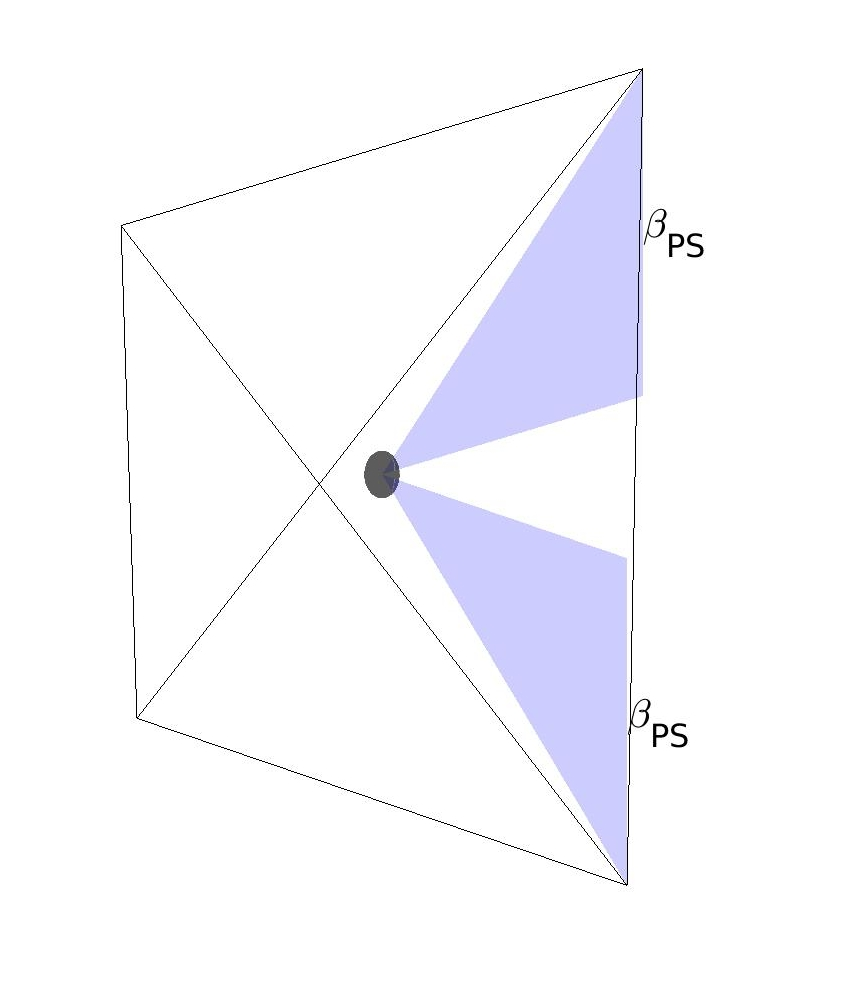
\includegraphics[width=\linewidth]{images/tetrahedron.jpg}
    \caption{Tetrahedron.} \label{fig:tetrahedron}
  \end{subfigure}
  \hspace*{\fill} % separation between the subfigures
  \begin{subfigure}[b]{0.27\textwidth}
    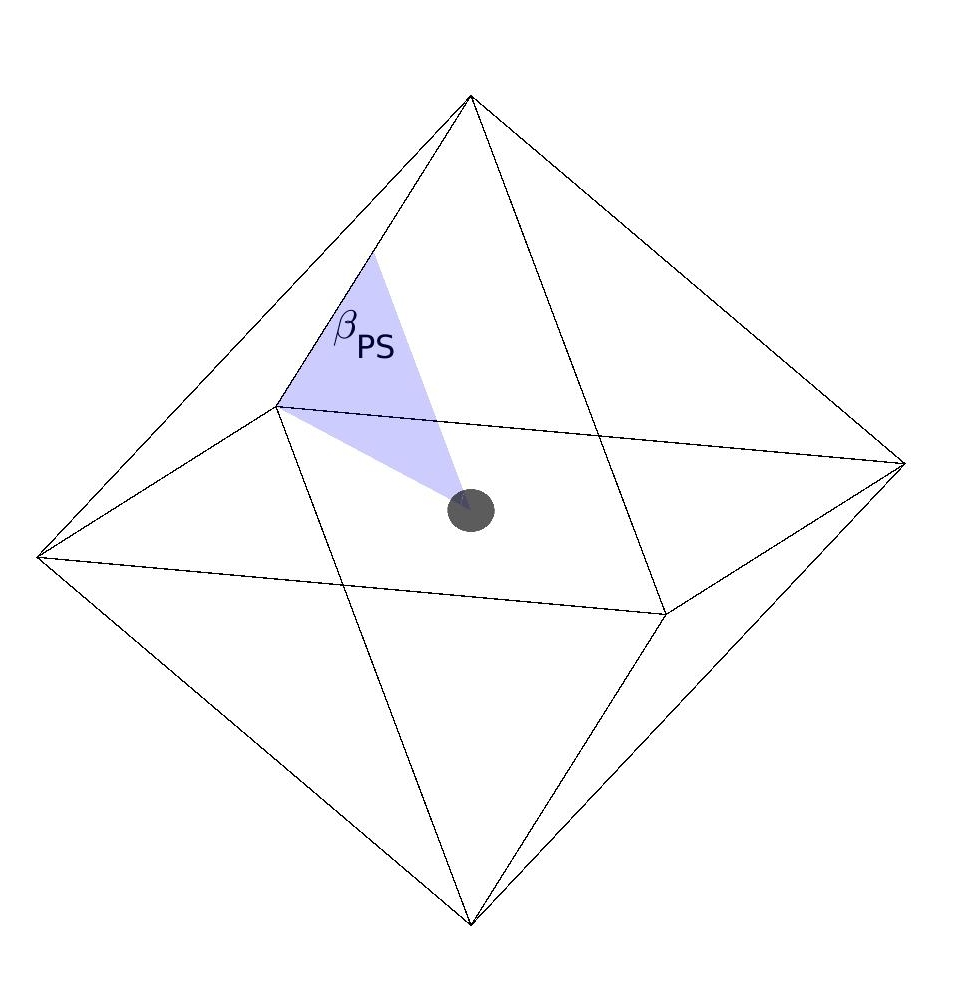
\includegraphics[width=\linewidth]{images/octahedron.jpg}
    \caption{Octahedron.} \label{fig:octahedron}
  \end{subfigure}
  \hspace*{\fill} % separation between the subfigures
  \begin{subfigure}[b]{0.26\textwidth}
    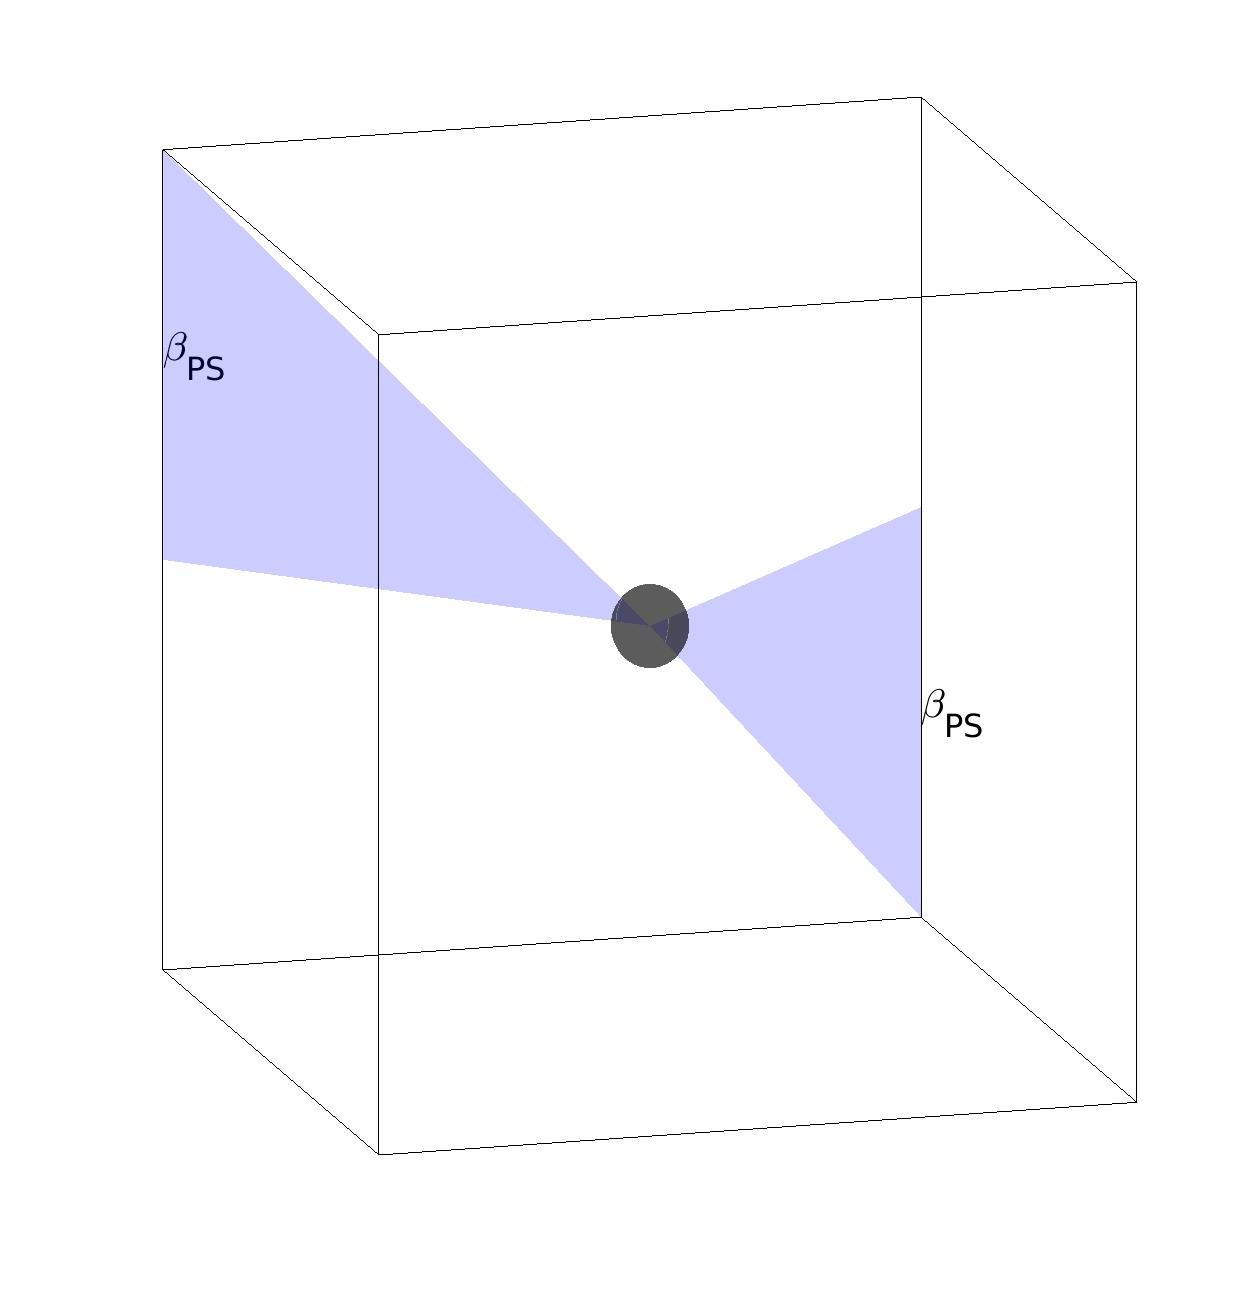
\includegraphics[width=\linewidth]{images/cube.jpg}
    \caption{Cube.} \label{fig:cube}
  \end{subfigure}
  \caption{The first three platonic solids $\big(\cos(\beta_{PS}) = \sqrt{\frac{2}{3}}
  \rightarrow \beta_{PS} \simeq 35.26^{\circ}\big)\, .$}
  \label{fig:platonic_solid}
\end{figure}

\section{Even Designs}
\label{sec:even_designs}

\subsection{Quad-copter}
\label{sec:quad_copter}

The first MAV morphology presented is obtained when optimizing to find
$\beta_{arm}$ and $\theta_{arm}$, with as fixed design parameters $n\ =\ 4$
and $L\ =\ 0.5\ [m]$ and as an initial solution $\beta_{arm,0} \ =\ [0^{\circ},
\  0^{\circ},\  0^{\circ},\ 0^{\circ}]$ and $\theta_{arm,0}\ =\
[0^{\circ},\  0^{\circ},\  0^{\circ},\  0^{\circ}]$. As a cost function for the
optimization problem, the cost function that maximizes the minimal attainable
force and the minimal attainable torque that the MAV can produce in any direction
and that minimizes the inertia of the drone is used. The result is depicted in
\Cref{fig:Quadcopter_1} and has the following features:

{\scriptsize\begin{itemize}
  \item $n\ =\ 4$
  \item $\beta_{arm}\ =\ [-32.42^{\circ},\  -35.49^{\circ},\  -35.44^{\circ},\  -35.49^{\circ}]$
  \item $\theta_{arm}\ =\ [-0.99^{\circ},\  -1.88^{\circ},\  -2.26^{\circ},\  -2.94^{\circ}]$
  \item $L\ =\ 0.5\ [m]$
\end{itemize}}

It is noticeable that the $\theta_{arm}$ tend towards zero and that the $\beta_{arm}$
tend towards the platonic solid angle $\beta_{PS}$. However, the design has not totally
converged. This is due to the fact that the optimization tool has, as mentioned in
\Cref{sec:limitations}, found a local minimum before reaching the global one,
which seems to be when the drone has the arms equally distributed in the horizontal
plane ($\theta_{arm}$ = 0) and forming the platonic solid angle with the same horizontal
plane ($\beta_{arm}\ =\ \beta_{PS}$). So as to verify this, the second
design is obtained when performing the same optimization as before with a slight
change, which consists in choosing as initial solution $\beta_{arm,0} \ =\
[35.26^{\circ},\  -35.26^{\circ},\  35.26^{\circ},\  -35.26^{\circ}]$. The result is
depicted in \Cref{fig:Quadcopter_1} and has the following parameters:

{\scriptsize\begin{itemize}
  \item $n\ =\ 4$
  \item $\beta_{arm}\ =\ [35.26^{\circ},\  -35.26^{\circ},\  35.26^{\circ},\  -35.26^{\circ}]$
  \item $\theta_{arm}\ =\ [0^{\circ},\  0^{\circ},\  0^{\circ},\  0^{\circ}]$
  \item $L\ =\ 0.5\ [m]$
\end{itemize}}

After optimization the second design is the same as the initial solution. This means
that the initially chosen design is optimal and it is very likely a global optimum
as when starting the optimization from different initial solution it converges to it.
It is interesting to note that the four propellers of the second design form the four
vertices of a tetrahedron (see \Cref{fig:Quadcopter_2_tetra}).

\begin{figure}[!ht]
  \resizebox{\textwidth}{!}{\begin{subfigure}[b]{0.5\textwidth}
    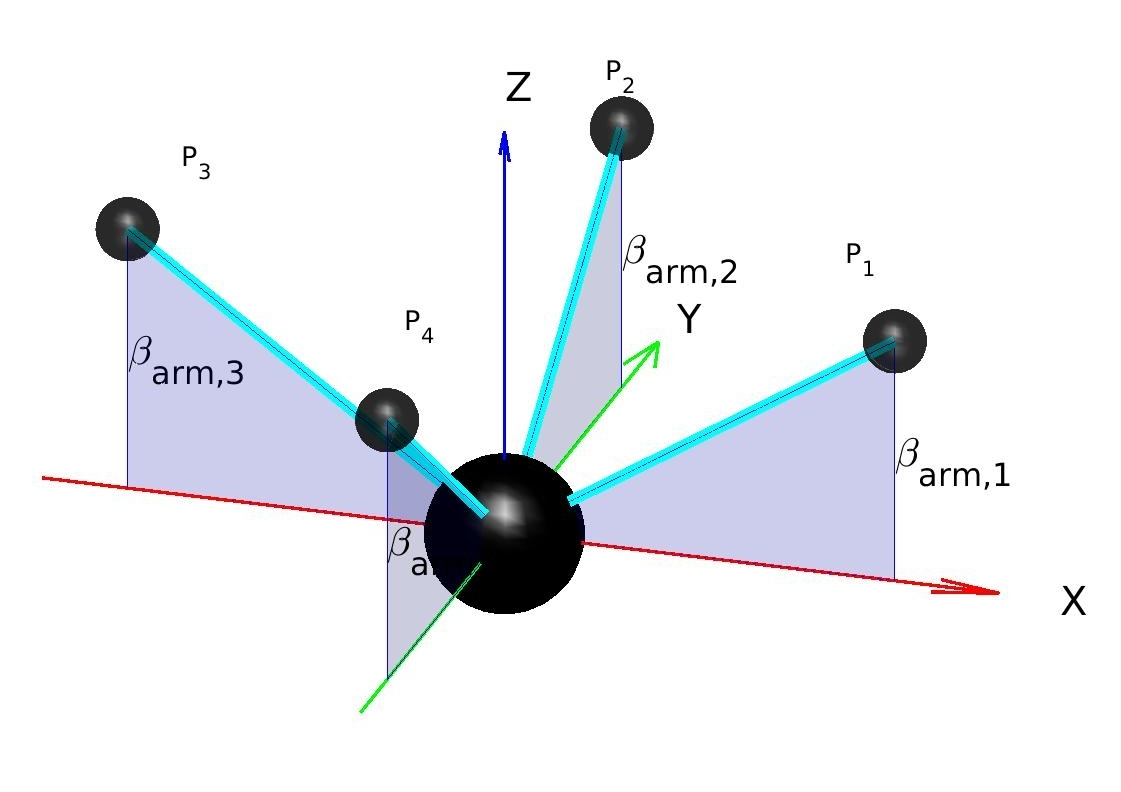
\includegraphics[width=\linewidth]{images/Quadcopter2.jpg}
    \caption{Design 1.} \label{fig:Quadcopter_1}
  \end{subfigure}
\hspace*{\fill} % separation between the subfigures
\begin{subfigure}[b]{0.45\textwidth}
    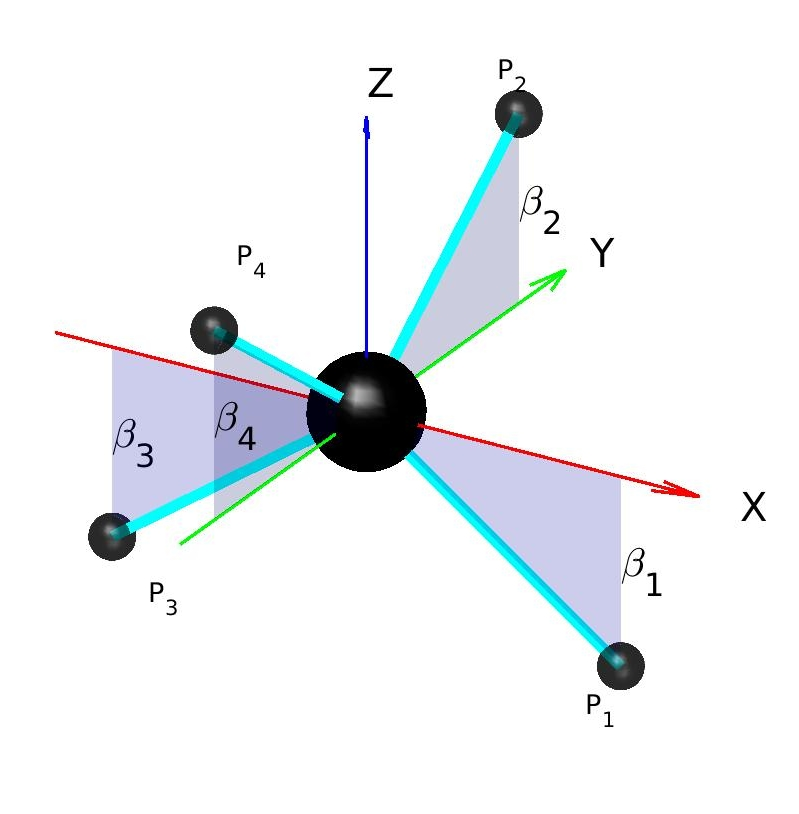
\includegraphics[width=\linewidth]{images/Quadcopter.jpg}
    \caption{Design 2.} \label{fig:Quadcopter_2}
  \end{subfigure}
  \hspace*{\fill} % separation between the subfigures
  \begin{subfigure}[b]{0.4\textwidth}
    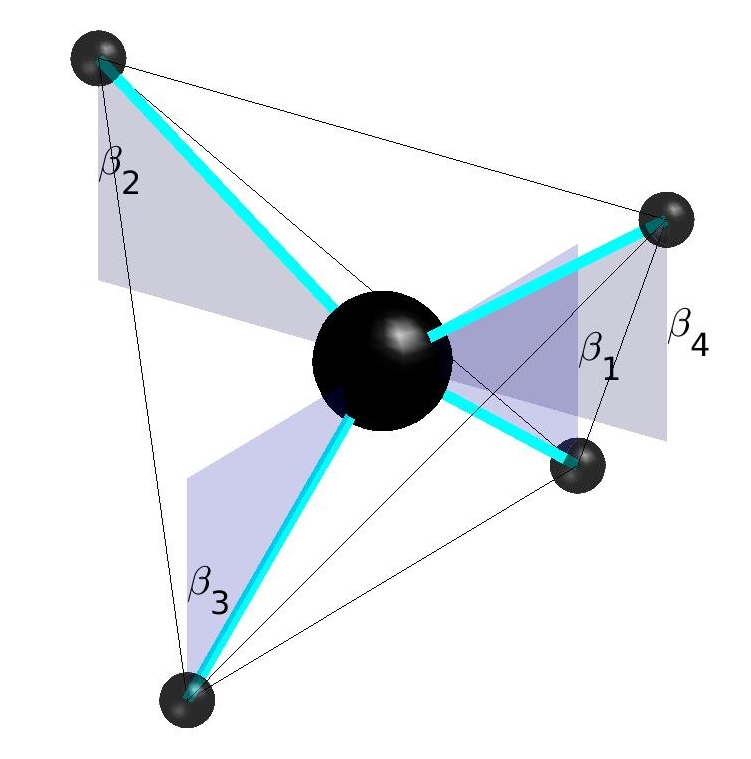
\includegraphics[width=\linewidth]{images/Quad_tetrahedron.jpg}
    \caption{Design 2 within a tetrahedron.} \label{fig:Quadcopter_2_tetra}
  \end{subfigure}}
  \caption{Representation of the designs obtained for the quad-copter.}
  \label{fig:Quadcopter_result}
\end{figure}

It is important to understand that for the tool, the designs with all the arms
on the same side (as design 1), or the designs with distributed arms (as design 2),
are equivalent. Even with slightly different arm angles’ magnitudes
between the two designs, when comparing \Cref{fig:Quadcopter1_spaces}with
\Cref{fig:Quadcopter2_spaces} and when comparing the different metrics
in \Cref{tab:tab_Quad_compare_force}, \Cref{tab:tab_Quad_compare_torque} and
\Cref{tab:tab_Quad_compare_hover}, one can easily see that the two designs
propose similar abilities. The main difference is the location of their center of mass
that the tool does not consider. For instance, second design’s CoM coincide with
the body origin. Which renders the drone more balanced and thus more controllable.

\begin{figure}[!ht]
  \begin{center}
  \resizebox{1.1\textwidth}{!}{\begin{subfigure}[b]{0.54\textwidth}
    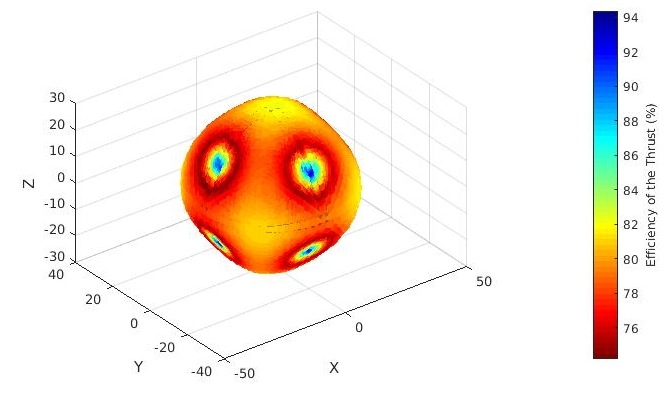
\includegraphics[width=\linewidth]{images/Quad_design_2_fspace.jpg}
    \caption{Attainable force space.} \label{fig:deisgn1_fspace}
  \end{subfigure}
  \hspace*{\fill} % separation between the subfigures
  \begin{subfigure}[b]{0.51\textwidth}
    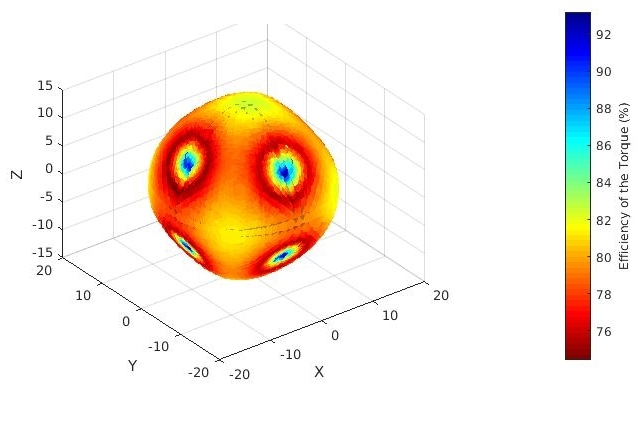
\includegraphics[width=\linewidth]{images/Quad_design_2_tspace.jpg}
    \caption{Attainable torque space.} \label{fig:deisgn1_tspace}
  \end{subfigure}
  \begin{subfigure}[b]{0.52\textwidth}
    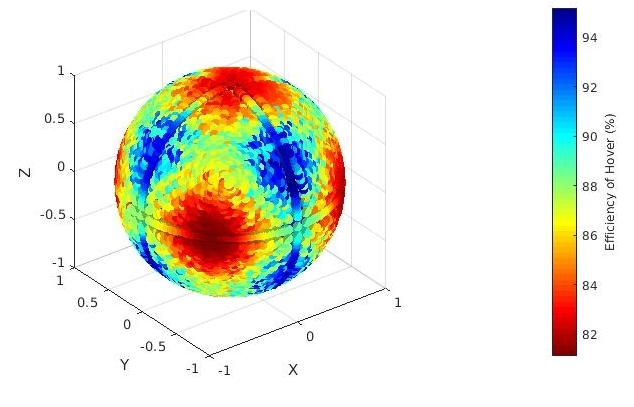
\includegraphics[width=\linewidth]{images/Quad_design_2_hspace.jpg}
    \caption{Hover efficiency in every orientation.} \label{fig:deisgn1_hspace}
  \end{subfigure}}
  \caption{Visual representation of the abilities of design 1.}
  \label{fig:Quadcopter1_spaces}
  \end{center}
\end{figure}

\begin{figure}[!ht]
  \begin{center}
  \resizebox{1.1\textwidth}{!}{\begin{subfigure}[b]{0.55\textwidth}
    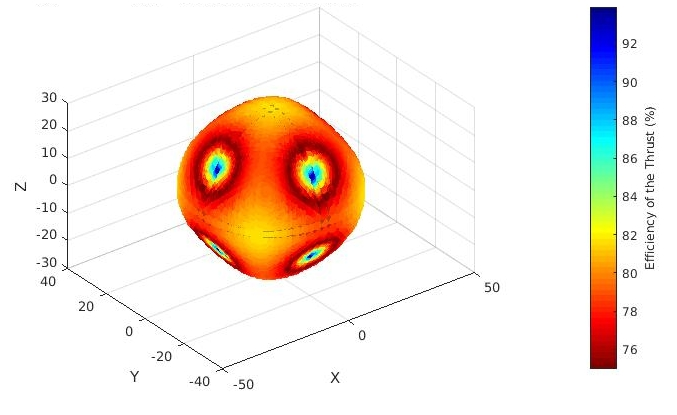
\includegraphics[width=\linewidth]{images/Quad_design_1_fspace.jpg}
    \caption{Attainable force space.} \label{fig:deisgn2_fspace}
  \end{subfigure}
  \hspace*{\fill} % separation between the subfigures
  \begin{subfigure}[b]{0.52\textwidth}
    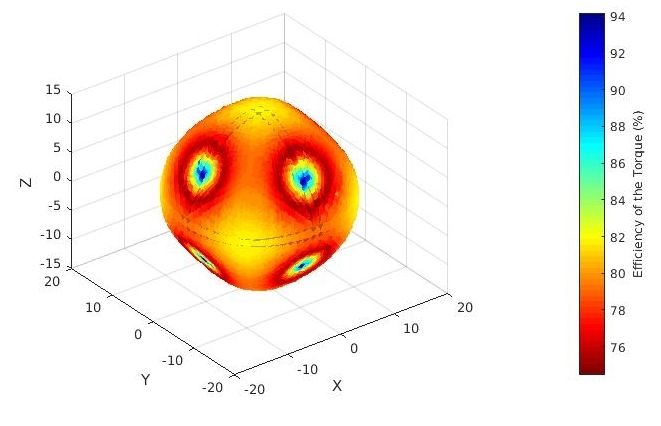
\includegraphics[width=\linewidth]{images/Quad_design_1_tspace.jpg}
    \caption{Attainable torque space.} \label{fig:deisgn2_tspace}
  \end{subfigure}
  \begin{subfigure}[b]{0.5\textwidth}
    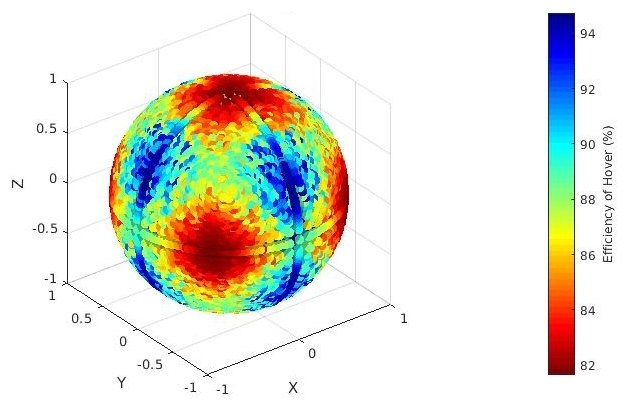
\includegraphics[width=\linewidth]{images/Quad_design_1_hspace.jpg}
    \caption{Hover efficiency in every orientation.} \label{fig:deisgn2_hspace}
  \end{subfigure}}
  \caption{Visual representation of the abilities of design 2.}
  \label{fig:Quadcopter2_spaces}
  \end{center}
\end{figure}

In the following tables, a comparison between the metrics of the optimal designs
and the standard quad-copter is proposed. Due to the tilting ability of the rotors,
the standard design is equally fully-actuated. Even though the force that the standard
quad-copter design can apply in the $Z$ direction is big, the forces that it can
apply on its side and in average are much more limited. We also notice that the
optimal designs proposed by the tool are actually meeting the omni-directionality
criteria stated in \Cref{sec:cost_functions}. Indeed, compared to the standard
design, the minimal forces and torques that the optimal designs can apply are high.
Furthermore, the volumes of the attainable forces and torques are big and shaped
like spheres, which makes the MAVs dynamical properties nearly invariant to their
orientation. Therefore it is not an overstatement to say that they are omni-directional.

\begin{table}[!ht]
\begin{center}
 \caption{Information on the designs’ force space properties.}\vspace{1ex}
 \label{tab:tab_Quad_compare_force}
 \resizebox{\textwidth}{!}{\begin{tabular}{|c|cccccc|}
 \hline
 Design & $F_{min}\ [N]$ & $F_{max}\ [N]$ & $F_{mean}\ [N]$ & $MAD(F)\ [N]$
 & Force space volume $[N^3]$& Force space surface $[N^2]$\\ \hline
  1 & 23.19 & 28.56 & 26.87 & 0.86 & 81'683 & 9'345\\
  2 & 23.23 & 28.37 & 26.87 & 0.86 & 81'710 & 9'326\\
  Standard & 17.37 & 34.74 & 24.43 & 3.43 & 65’673 & 8’865\\
 \hline
 \end{tabular}}
\end{center}
\end{table}

\begin{table}[!ht]
\begin{center}
 \caption{Information on the designs’ torque space properties.}\vspace{1ex}
 \label{tab:tab_Quad_compare_torque}
 \resizebox{\textwidth}{!}{\begin{tabular}{|c|cccccc|}
 \hline
 Design & $M_{min}\ [Nm]$ & $M_{max}\ [Nm]$ & $M_{mean}\ [Nm]$ & $MAD(M)\ [Nm]$
 & Torque space volume $[N^3m^3]$ & Torque space surface $[N^2m^2]$\\ \hline
 1 & 11.62 & 14.32 & 13.47 & 0.43 & 10'298 & 2'355\\
 2 & 11.65 & 14.23 & 13.47 & 0.43 & 10'300 & 2'348\\
 Standard & 8.7 & 17.42 & 12.25 & 1.72 & 8’284 & 2’219\\
 \hline
 \end{tabular}}
\end{center}
\end{table}

\begin{table}[!ht]
\begin{center}
 \caption{Information on the designs’ hover efficiency space properties.}\vspace{1ex}
 \label{tab:tab_Quad_compare_hover}
 {\scriptsize\begin{tabular}{|c|cccc|}
 \hline
  Design & $H_{eff,min}\ [\%]$ & $H_{eff,max}\ [\%]$ & $H_{eff,mean}\ [\%]$
  & $MAD(H_{eff})\ [\%]$\\ \hline
  1 & 81.11 & 95.18 & 87.03 & 2.63\\
  2 & 81.65 & 94.73 & 87.1 & 2.6\\
  Standard & 70.7 & 100 & 82.3 & 6.1\\
 \hline
\end{tabular}}
\end{center}
\end{table}

\subsection{Hexa-copter}
\label{sec:hexa_copter}

When optimizing to find $\beta_{arm}$ and $\theta_{arm}$, with fixed
design parameters $n\ =\ 6$ and $L\ =\ 0.5\ [m]$ and as chosen cost function
for the optimization problem the cost function that maximizes the volumes
of the force and torque spaces, the tool returns a design defined by:

{\scriptsize\begin{itemize}
  \item $n\ =\ 6$
  \item $\beta_{arm}\ =\ [35.26^{\circ},\  -35.26^{\circ},\  35.26^{\circ},\  -35.26^{\circ},\
                          35.26^{\circ},\  -35.26^{\circ}]$
  \item $\theta_{arm}\ =\ [0^{\circ},\  0^{\circ},\  0^{\circ},\  0^{\circ},\ 0^{\circ},\  0^{\circ}]$
  \item $L\ =\ 0.5\ [m]$
\end{itemize}}

It is noteworthy that even when using a different cost function to solve
tho omni-directionality optimization problem, the arm angles $\beta_{arm}$
converge to the platonic solid angle and that the propeller tend to from the
platonic solid that matches their number. For instance, in this six propeller case
the optimal MAV design form an octahedron (see \Cref{fig:Hexacopter_resultb}).
In the rest of this section the optimal drone design depicted in
\Cref{fig:Hexacopter_resulta} is compared to the standard hexa-copter design,
which is equivalent to Voliro presented in \citep{kamel_voliro:_2018}
(see \Cref{fig:Hexacopter_resultc}).

\begin{figure}[!ht]
  \resizebox{\textwidth}{!}{\begin{subfigure}[b]{0.6\textwidth}
    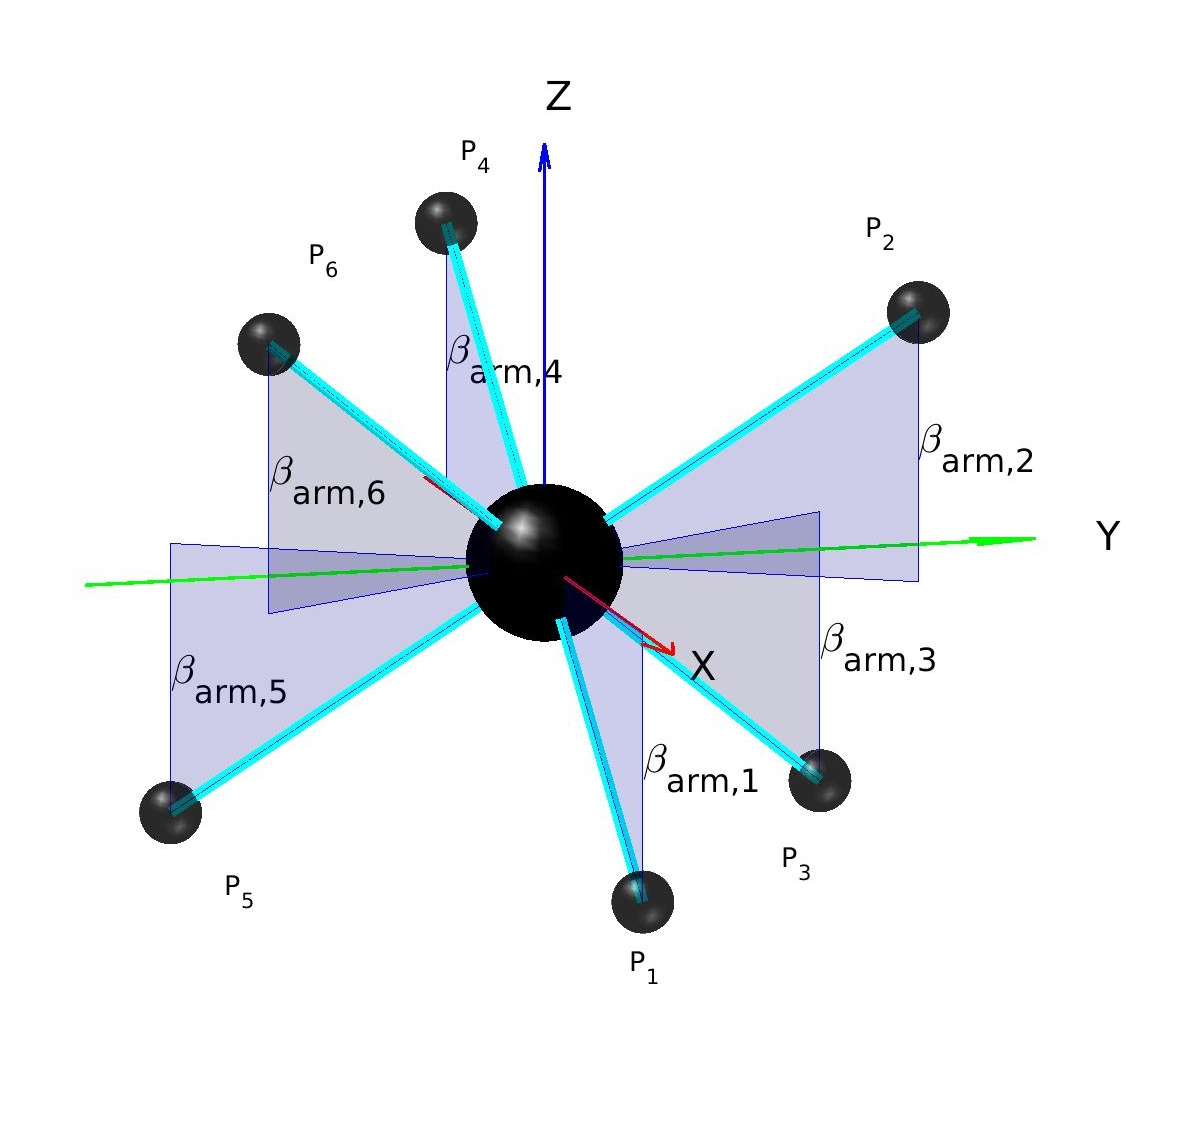
\includegraphics[width=\linewidth]{images/Hexacopter.jpg}
    \caption{Optimal hexa-copter} \label{fig:Hexacopter_resulta}
  \end{subfigure}
  \hspace*{\fill} % separation between the subfigures
  \begin{subfigure}[b]{0.55\textwidth}
    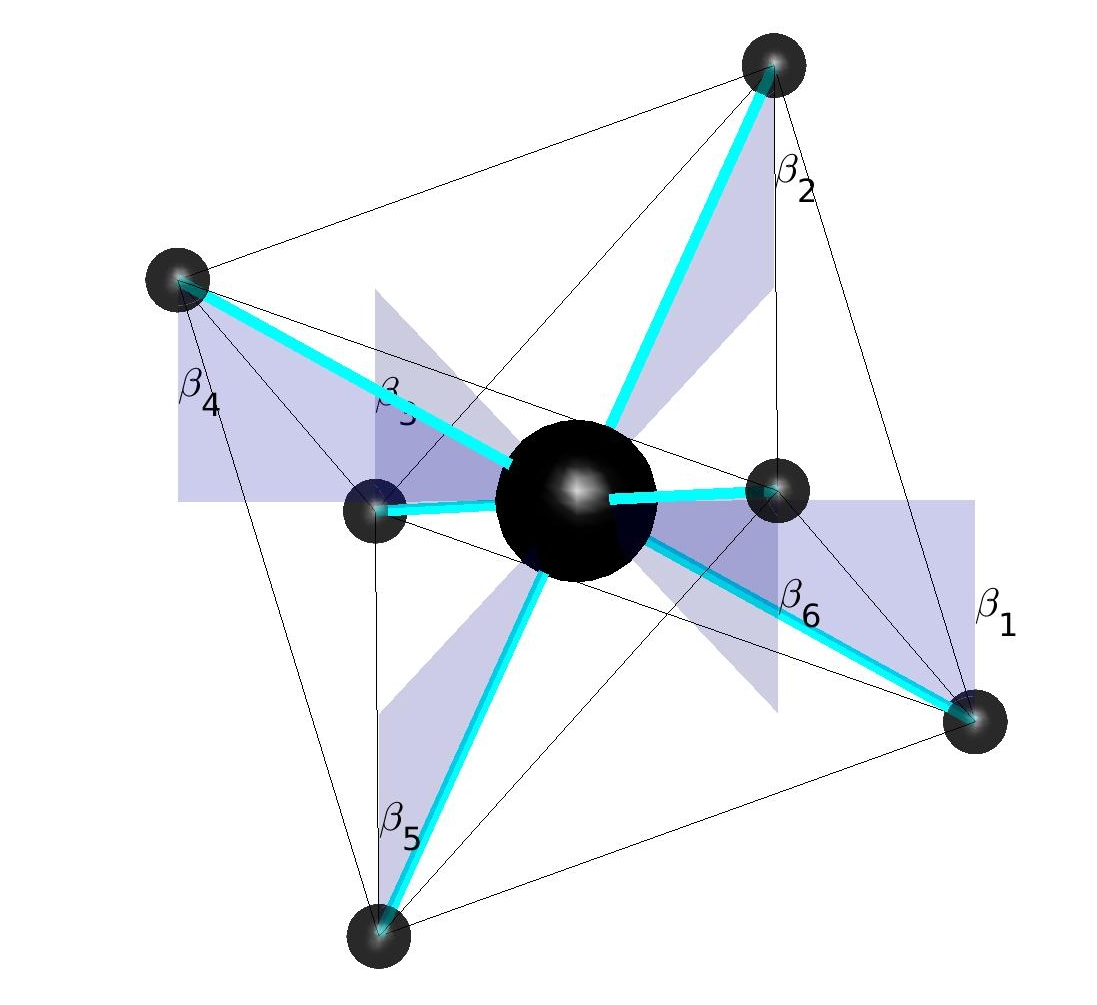
\includegraphics[width=\linewidth]{images/Hexa_octahedron.jpg}
    \caption{Optimal hexa-copter within an octahedron.} \label{fig:Hexacopter_resultb}
  \end{subfigure}
  \hspace*{\fill} % separation between the subfigures
  \begin{subfigure}[b]{0.8\textwidth}
    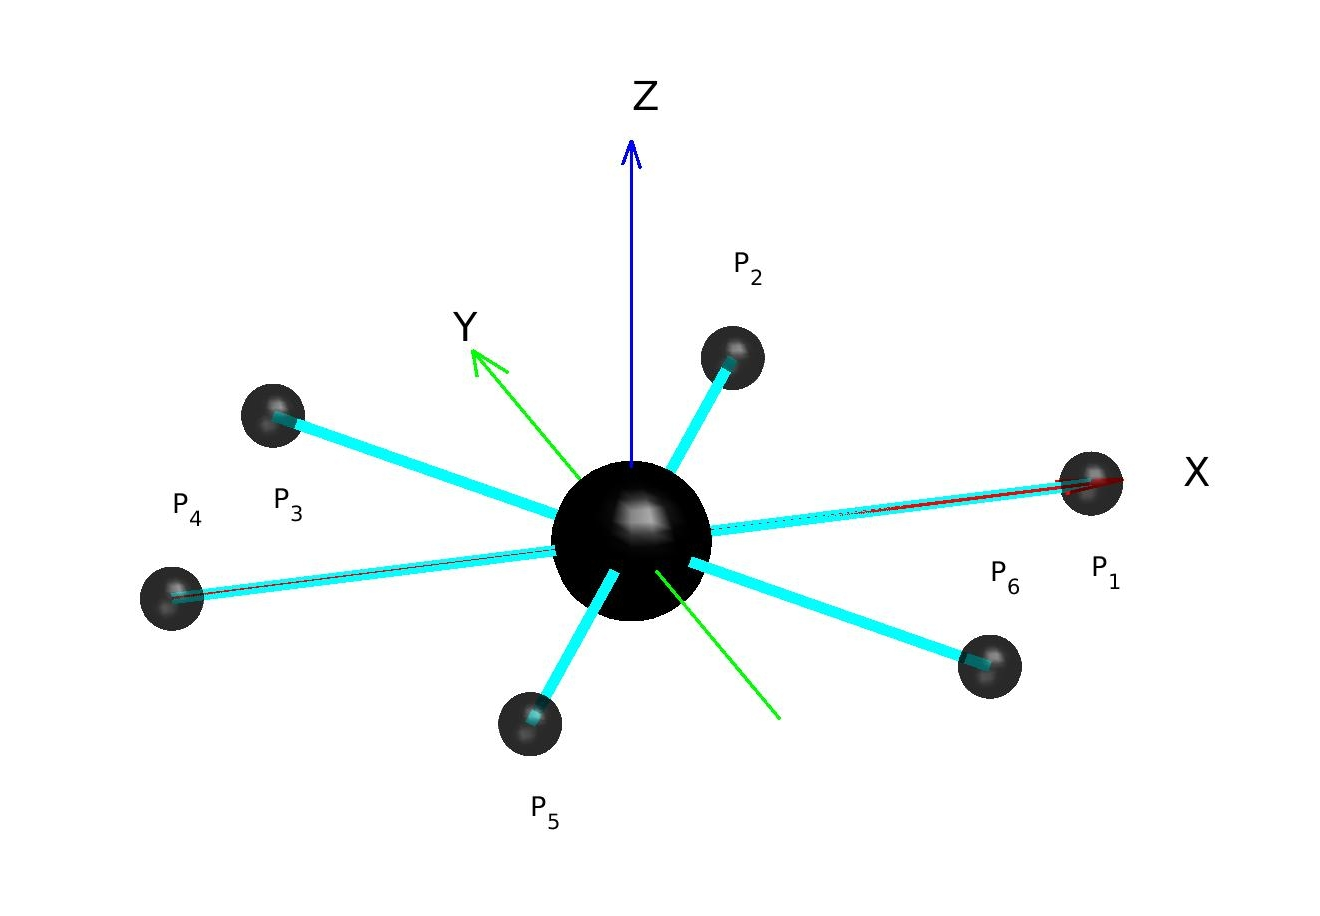
\includegraphics[width=\linewidth]{images/Voliro.jpg}
    \caption{Voliro's design for comparison.} \label{fig:Hexacopter_resultc}
  \end{subfigure}}
  \caption{Representation of the design obtained for the hexa-copter.}
  \label{fig:Hexacopter_result}
\end{figure}

\begin{figure}[!ht]
  \resizebox{\textwidth}{!}{\begin{subfigure}[b]{0.44\textwidth}
    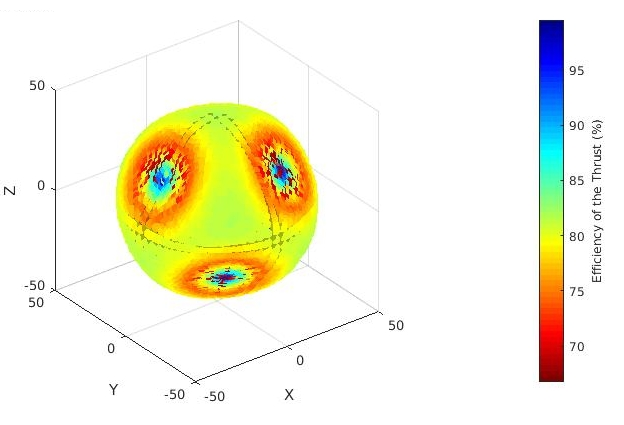
\includegraphics[width=\linewidth]{images/Hexa_fspace.jpg}
    \caption{Attainable force space.} \label{fig:hexa_fspace}
  \end{subfigure}
  \hspace*{\fill} % separation between the subfigures
  \begin{subfigure}[b]{0.46\textwidth}
    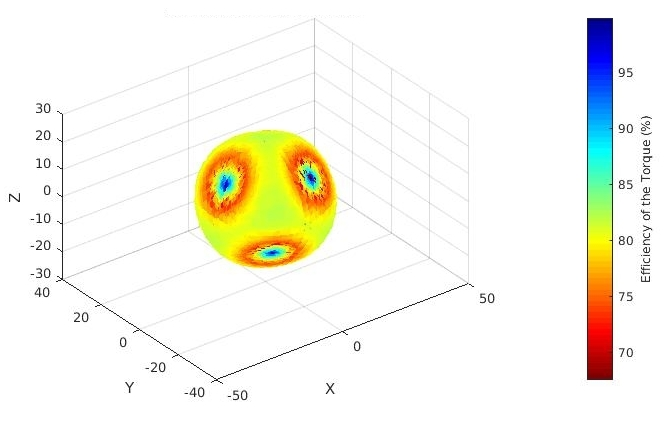
\includegraphics[width=\linewidth]{images/Hexa_tspace.jpg}
    \caption{Attainable torque space.} \label{fig:hexa_tspace}
  \end{subfigure}
  \begin{subfigure}[b]{0.47\textwidth}
    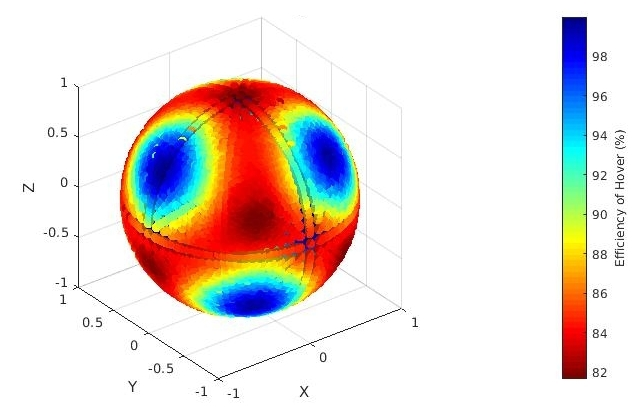
\includegraphics[width=\linewidth]{images/Hexa_hspace.jpg}
    \caption{Hover efficiency in every orientation.} \label{fig:hexa_hspace}
  \end{subfigure}}
  \caption{Visual representation of the abilities of the optimal hexa-copter.}
  \label{fig:Hexacopter_spaces}
\end{figure}

\begin{figure}[!ht]
  \resizebox{\textwidth}{!}{\begin{subfigure}[b]{0.52\textwidth}
    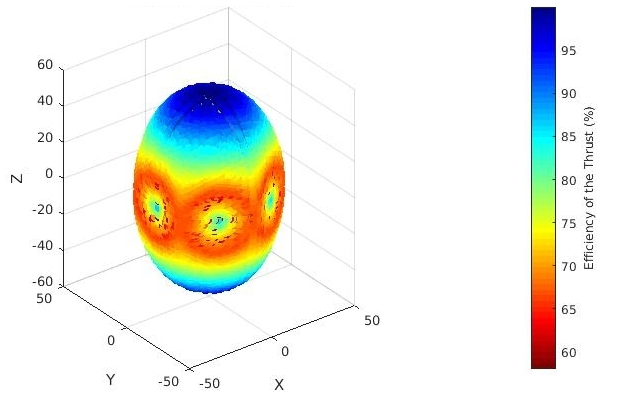
\includegraphics[width=\linewidth]{images/Voliro_fspace.jpg}
    \caption{Attainable force space.} \label{fig:voliro_fspace}
  \end{subfigure}
  \hspace*{\fill} % separation between the subfigures
  \begin{subfigure}[b]{0.5\textwidth}
    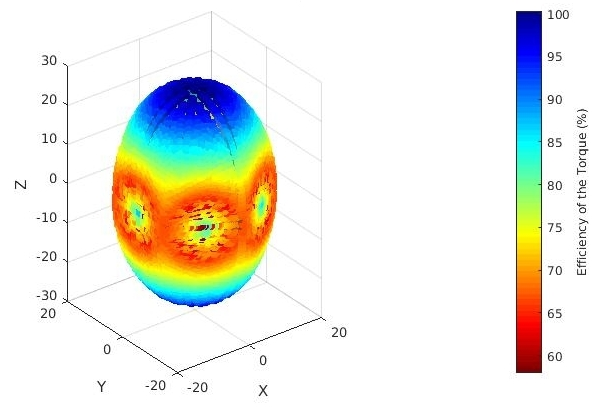
\includegraphics[width=\linewidth]{images/Voliro_tspace.jpg}
    \caption{Attainable torque space.} \label{fig:voliro_tspace}
  \end{subfigure}
  \begin{subfigure}[b]{0.52\textwidth}
    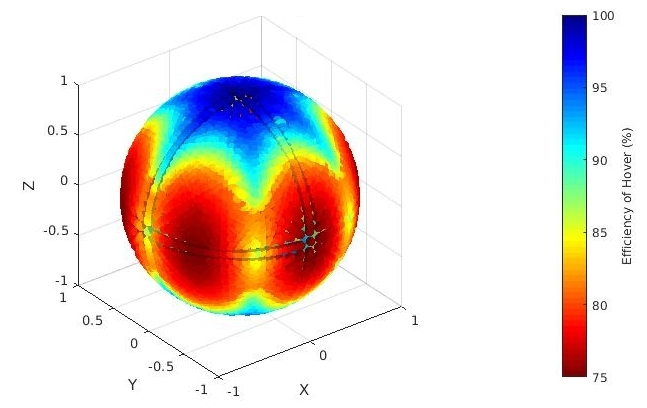
\includegraphics[width=\linewidth]{images/Voliro_hspace.jpg}
    \caption{Hover efficiency in every orientation.} \label{fig:voliro_hspace}
  \end{subfigure}}
  \caption{Visual representation of the abilities of Voliro.}
  \label{fig:Voliro_spaces}
\end{figure}

When comparing the different spaces shown in \Cref{fig:Hexacopter_spaces}
and in \Cref{fig:Voliro_spaces}, the first noticeable thing is that the torque
and force spaces of the optimal hexa-copter are much more spherical than
Voliro’s. Which makes the optimal hexa-copter’s dynamical features more
independent form its orientation. Then, one can without difficulty notice in
\Cref{fig:voliro_hspace} that Voliro can only hover with a $100\ \%$ efficiency
when oriented near the initial position or upside down. Whereas the obtained
design can hover with a $100\ \%$ efficiency in at least six very different orientations
(see \Cref{fig:hexa_hspace}). Furthermore, the hover efficiency is generally
higher for the optimized design (see \Cref{tab:tab_Hexa_compare_hover}).

\begin{table}[!ht]
\begin{center}
 \caption{Information on the designs’ force space properties.}\vspace{1ex}
 \label{tab:tab_Hexa_compare_force}
 \resizebox{\textwidth}{!}{\begin{tabular}{|c|cccccc|}
 \hline
 Design & $F_{min}\ [N]$ & $F_{max}\ [N]$ & $F_{mean}\ [N]$ & $MAD(F)\ [N]$
 & Force space volume $[N^3]$& Force space surface $[N^2]$\\ \hline
 Optimal hexa-copter & 34.74 & 42.55 & 39.52 & 2.21 & 267'010 & 20'922\\
 Voliro & 26.6 & 52.11 & 37.77 & 4.33 & 244'293 & 20'170\\
 \hline
 \end{tabular}}
\end{center}
\end{table}

\begin{table}[!ht]
\begin{center}
 \caption{Information on the designs’ torque space properties.}\vspace{1ex}
 \label{tab:tab_Hexa_compare_torque}
 \resizebox{\textwidth}{!}{\begin{tabular}{|c|cccccc|}
 \hline
 Design & $M_{min}\ [Nm]$ & $M_{max}\ [Nm]$ & $M_{mean}\ [Nm]$ & $MAD(M)\ [Nm]$
 & Torque space volume $[N^3m^3]$ & Torque space surface $[N^2m^2]$\\ \hline
 Optimal hexa-copter & 17.42 & 21.34 & 19.82 & 1.1 & 33'687 & 5'230\\
 Voliro & 15.09 & 26.13 & 18.94 & 2.17 & 30'788 & 5'121\\
 \hline
 \end{tabular}}
\end{center}
\end{table}

\begin{table}[!ht]
\begin{center}
 \caption{Information on the designs’ hover efficiency space properties.}\vspace{1ex}
 \label{tab:tab_Hexa_compare_hover}
 {\scriptsize\begin{tabular}{|c|cccc|}
 \hline
  Design & $H_{eff,min}\ [\%]$ & $H_{eff,max}\ [\%]$ & $H_{eff,mean}\ [\%]$
  & $MAD(H_{eff})\ [\%]$\\ \hline
  Optimal hexa-copter & 81.65 & 100 & 88.92 & 4.43\\
  Voliro & 75 & 100 & 84.21 & 5.35\\
 \hline
\end{tabular}}
\end{center}
\end{table}

\clearpage

\subsection{Octa-copter}
\label{sec:octa_copter}

The next result is obtained when the tool solves the optimization problem
for an eight rotor MAV, with as a cost function, the one that maximizes the
minimal attainable force and the minimal attainable torque that the MAV
can produce in any direction and that minimizes the inertia of the drone.
The result represented in \Cref{fig:Octacopter_resulta} is defined by:

{\scriptsize\begin{itemize}
  \item $n\ =\ 8$
  \item $\beta_{arm}\ =\ [35.26^{\circ},\  -35.26^{\circ},\  35.26^{\circ},\  -35.26^{\circ},\
                          35.26^{\circ},\  -35.26^{\circ},\ 35.26^{\circ},\  -35.26^{\circ}]$
  \item $\theta_{arm}\ =\ [0^{\circ},\  0^{\circ},\  0^{\circ},\  0^{\circ},\ 0^{\circ},\  0^{\circ},\ 0^{\circ},\  0^{\circ}]$
  \item $L\ =\ 0.5\ [m]$
\end{itemize}}

The morphology converged once more to an even distribution of the arms in
the horizontal plane and to $\beta_{arm}$ equal to plus or minus $\beta_{PS}$
Out of curiosity the obtained result is compared to the Omnicopter presented  in
\citep{brescianini_design_2016}. However, for the sake of a meaningful
comparison, it is assumed that the Omnicopter can dynamically tilt its rotors
around their axes (see \Cref{fig:Octacopter_resultb}). The Omnicopter design
parameters are:

{\scriptsize\begin{itemize}
  \item $n\ =\ 8$
  \item $\beta_{arm}\ =\ [-35.26^{\circ},\  -35.26^{\circ},\  -35.26^{\circ},\  -35.26^{\circ},\
                          35.26^{\circ},\  35.26^{\circ},\ 35.26^{\circ},\  35.26^{\circ}]$
  \item $\theta_{arm}\ =\ [0^{\circ},\  45^{\circ},\  90^{\circ},\  135^{\circ},\
                          180^{\circ},\  -135^{\circ},\ -90^{\circ},\  -45^{\circ}]$
  \item $L\ =\ 0.5\ [m]$
\end{itemize}}

\begin{figure}[!ht]
  \resizebox{\textwidth}{!}{\begin{subfigure}[b]{0.6\textwidth}
    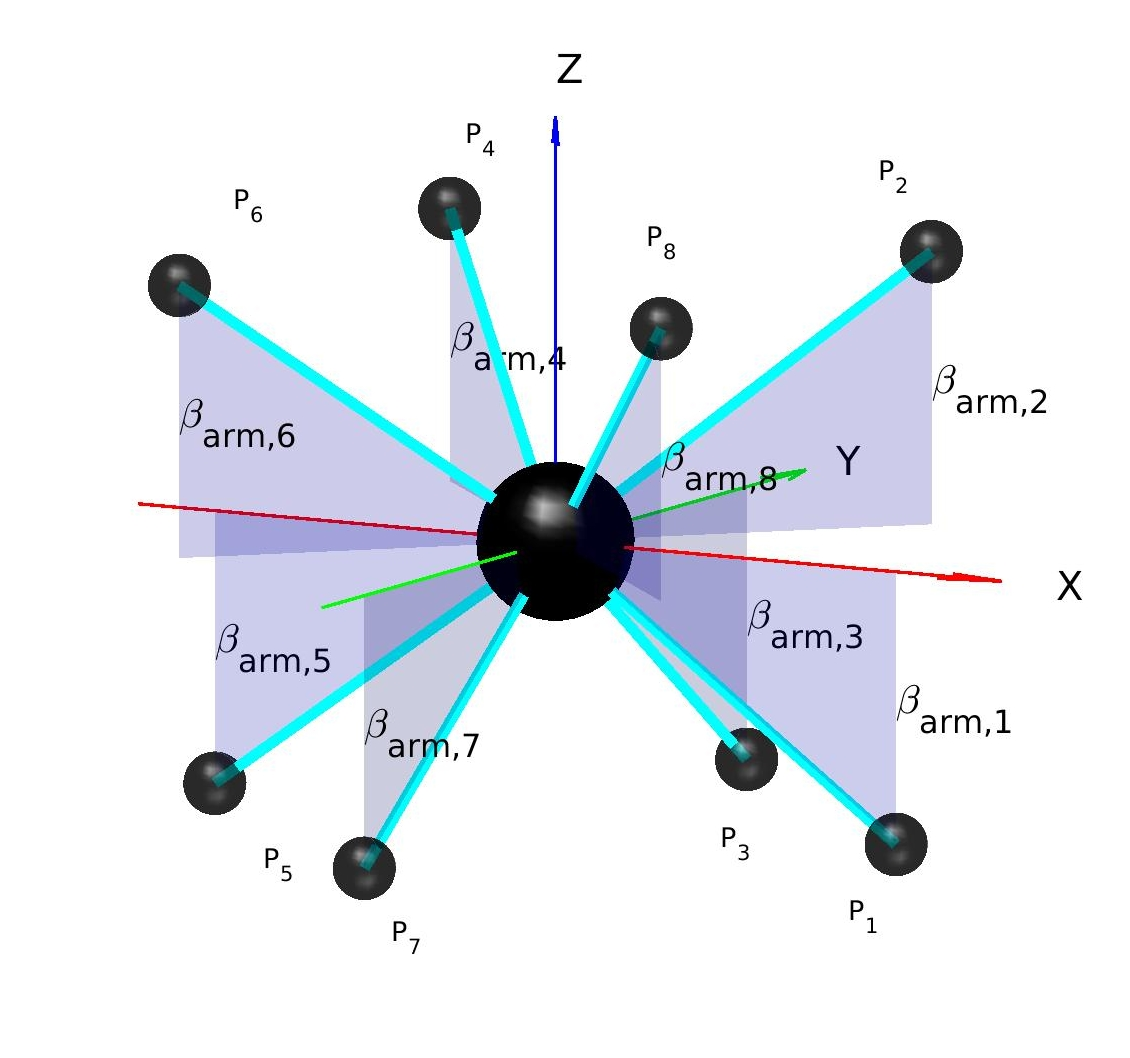
\includegraphics[width=\linewidth]{images/Octacopter.jpg}
    \caption{Optimal hexa-copter} \label{fig:Octacopter_resulta}
  \end{subfigure}
  \hspace*{\fill} % separation between the subfigures
  \begin{subfigure}[b]{0.6\textwidth}
    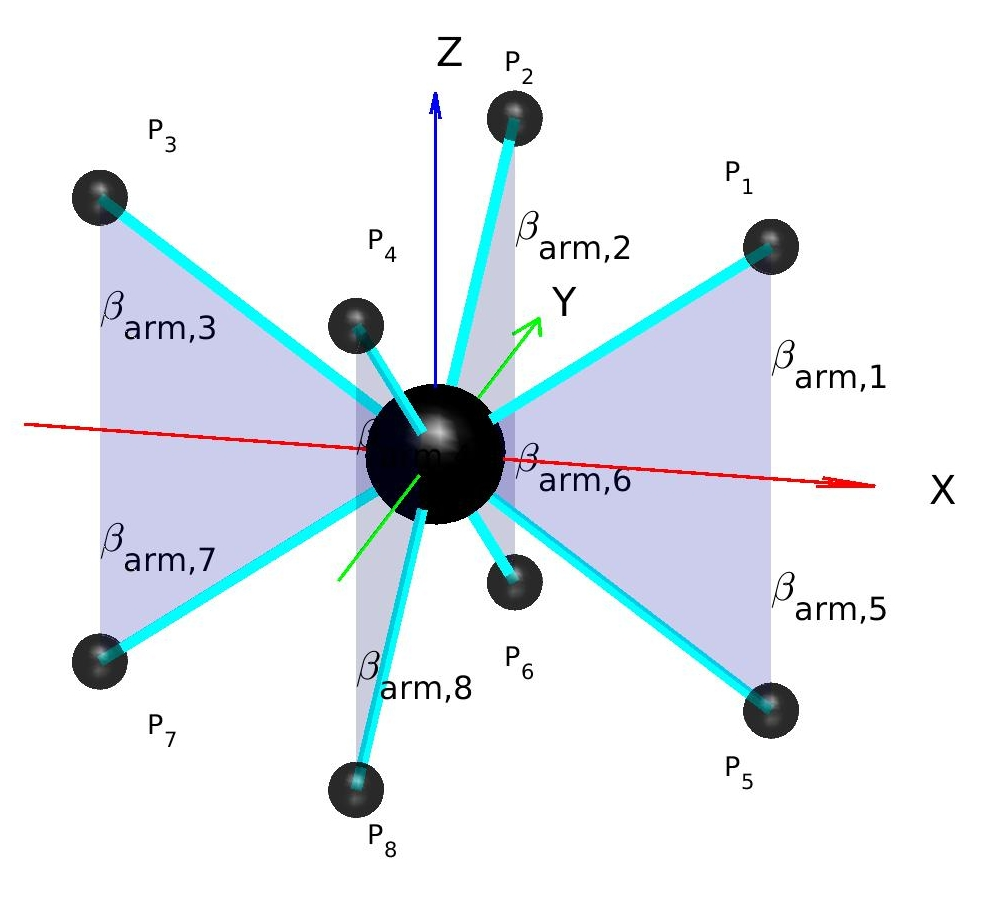
\includegraphics[width=\linewidth]{images/omnicopter.jpg}
    \caption{Omnicopter's design for comparison.} \label{fig:Octacopter_resultb}
  \end{subfigure}
  \hspace*{\fill} % separation between the subfigures
  \begin{subfigure}[b]{0.5\textwidth}
    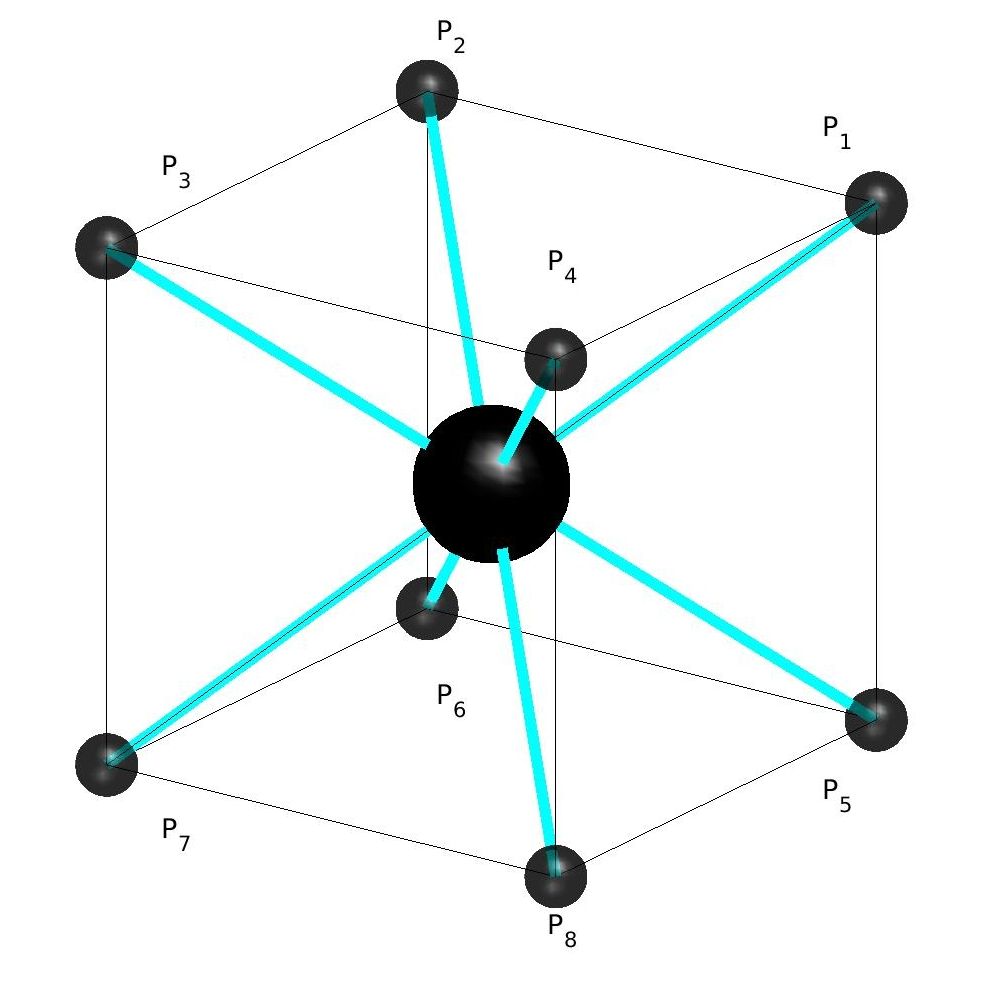
\includegraphics[width=\linewidth]{images/Octa_cube.jpg}
    \caption{Omnicopter in a cube.} \label{fig:Octacopter_resultc}
  \end{subfigure}}
  \caption{Representation of the designs obtained for the octa-copter.}
  \label{fig:Octacopter_result}
\end{figure}

It is interesting to note that this time the design returned by the tool does not
form a platonic solid with its propellers, but the Omnicopter does (see
\Cref{fig:Octacopter_resultc}).

\begin{figure}[!ht]
  \resizebox{\textwidth}{!}{\begin{subfigure}[b]{0.55\textwidth}
    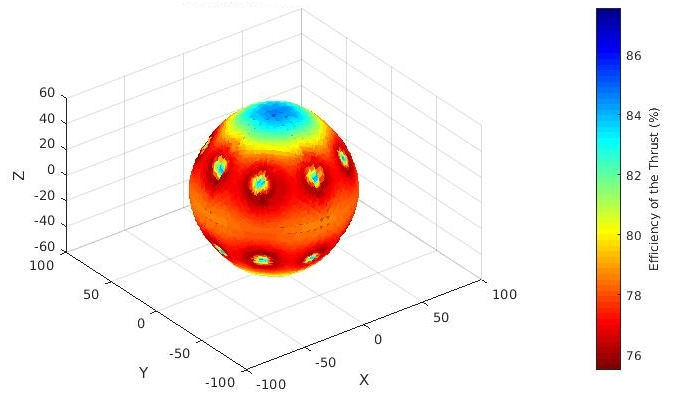
\includegraphics[width=\linewidth]{images/Octa_fspace.jpg}
    \caption{Attainable force space.} \label{fig:Octa_fspace}
  \end{subfigure}
  \hspace*{\fill} % separation between the subfigures
  \begin{subfigure}[b]{0.5\textwidth}
    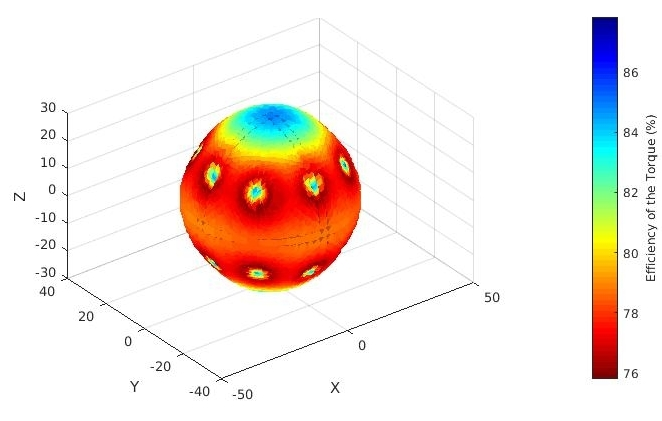
\includegraphics[width=\linewidth]{images/Octa_tspace.jpg}
    \caption{Attainable torque space.} \label{fig:Octa_tspace}
  \end{subfigure}
  \begin{subfigure}[b]{0.45\textwidth}
    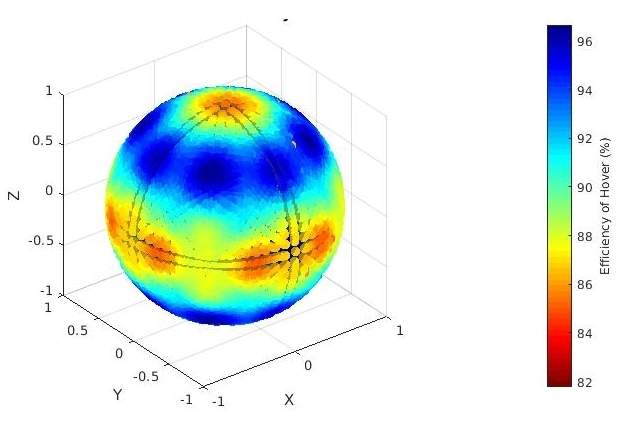
\includegraphics[width=\linewidth]{images/Octa_hspace.jpg}
    \caption{Hover efficiency in every orientation.} \label{fig:Octa_hspace}
  \end{subfigure}}
  \caption{Visual representation of the abilities of the optimal octa-copter.}
  \label{fig:Octacopter_spaces}
\end{figure}

\begin{figure}[!ht]
  \resizebox{\textwidth}{!}{\begin{subfigure}[b]{0.55\textwidth}
    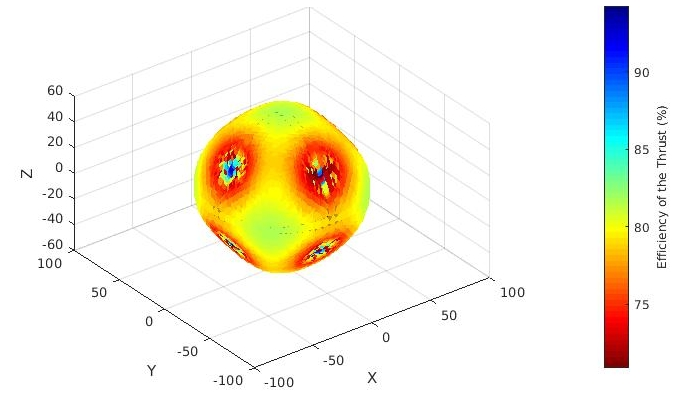
\includegraphics[width=\linewidth]{images/Omnicopter_fspace.jpg}
    \caption{Attainable force space.} \label{fig:Omnicopter_fspace}
  \end{subfigure}
  \hspace*{\fill} % separation between the subfigures
  \begin{subfigure}[b]{0.5\textwidth}
    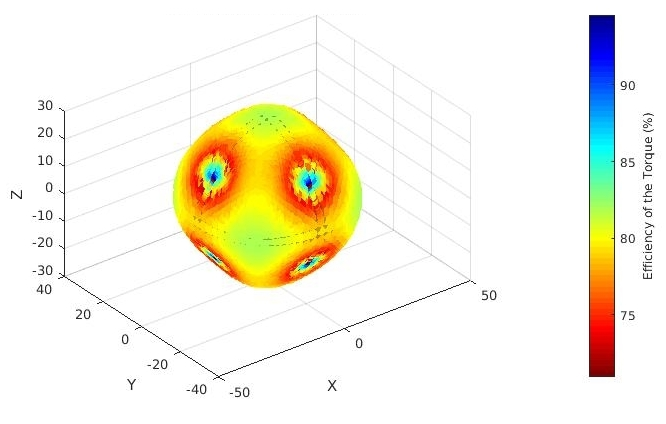
\includegraphics[width=\linewidth]{images/Omnicopter_tspace.jpg}
    \caption{Attainable torque space.} \label{fig:Omnicopter_tspace}
  \end{subfigure}
  \begin{subfigure}[b]{0.45\textwidth}
    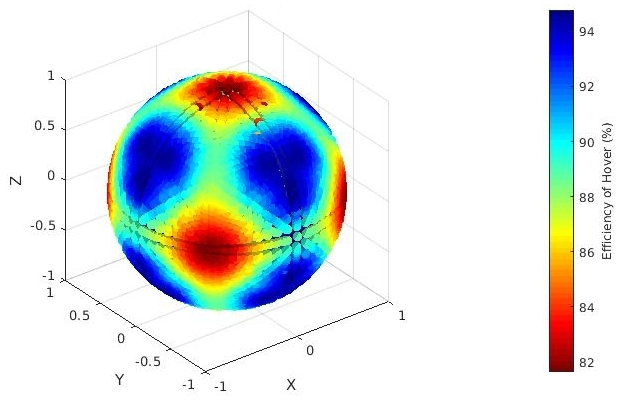
\includegraphics[width=\linewidth]{images/Omnicopter_hspace.jpg}
    \caption{Hover efficiency in every orientation.} \label{fig:Omnicopter_hspace}
  \end{subfigure}}
  \caption{Visual representation of the abilities of the Omnicopter.}
  \label{fig:Omnicopter_spaces}
\end{figure}

When comparing the two designs’ features represented in \Cref{fig:Omnicopter_spaces}
and \Cref{fig:Octacopter_spaces} and detailed in \Cref{tab:tab_Octa_compare_force},
\Cref{tab:tab_Octa_compare_torque} and \Cref{tab:tab_Octa_compare_hover}, one
notices that the two design are quite similar. Nevertheless, the arms of the optimal octa-copter
are more evenly distributed, this leads to a slightly bigger torque and force space volume
and a average hover efficiency better for the optimal octa-copter.

\begin{table}[!ht]
\begin{center}
 \caption{Information on the designs’ force space properties.}\vspace{1ex}
 \label{tab:tab_Octa_compare_force}
 \resizebox{\textwidth}{!}{\begin{tabular}{|c|cccccc|}
 \hline
 Design & $F_{min}\ [N]$ & $F_{max}\ [N]$ & $F_{mean}\ [N]$ & $MAD(F)\ [N]$
 & Force space volume $[N^3]$& Force space surface $[N^2]$\\ \hline
 Optimal octa-copter & 44.7 & 58.78 & 53.95 & 0.94 & 669'339 & 37'625\\
 Omnicopter & 46.46 & 56.73 & 53.75 & 1.72 & 653'736 & 37'263\\
 \hline
 \end{tabular}}
\end{center}
\end{table}

\begin{table}[!ht]
\begin{center}
 \caption{Information on the designs’ torque space properties.}\vspace{1ex}
 \label{tab:tab_Octa_compare_torque}
 \resizebox{\textwidth}{!}{\begin{tabular}{|c|cccccc|}
 \hline
 Design & $M_{min}\ [Nm]$ & $M_{max}\ [Nm]$ & $M_{mean}\ [Nm]$ & $MAD(M)\ [Nm]$
 & Torque space volume $[N^3m^3]$ & Torque space surface $[N^2m^2]$\\ \hline
 Optimal octa-copter & 22.4 & 29.48 & 27 & 0.47 & 84'417 & 9'463\\
 Omnicopter & 23.3 & 28.45 & 26.95 & 0.86 & 82'446 & 9'374\\
 \hline
 \end{tabular}}
\end{center}
\end{table}

{\scriptsize\begin{table}[!ht]
\begin{center}
 \caption{Information on the designs’ hover efficiency space properties.}\vspace{1ex}
 \label{tab:tab_Octa_compare_hover}
 {\scriptsize\begin{tabular}{|c|cccc|}
 \hline
  Design & $H_{eff,min}\ [\%]$ & $H_{eff,max}\ [\%]$ & $H_{eff,mean}\ [\%]$
  & $MAD(H_{eff})\ [\%]$\\ \hline
  Optimal octa-copter & 81.78 & 96.65 & 91.42 & 2.7\\
  Omnicopter & 81.64 & 94.77 & 89.36 & 2.82\\
 \hline
\end{tabular}}
\end{center}
\end{table}}

\clearpage

\section{Odd Designs}
\label{sec:odd_designs}

\subsection{Penta-copter}
\label{sec:penta_copter}

The next MAV design presented is interesting, indeed, the optimization tool
converged to an optimal solution, which is very odd. This result was obtained
when solving the morphology optimization problem for a five-rotors drone,
with as a cost function, the one that maximizes the force, the torque and the
hover efficiency in all directions. For this optimization, $\beta_{arm,1}$
$\beta_{arm,2}$ and $\theta_{arm,1}$ are forced to be zero,
in order for the tool to have less parameters to optimize and thus to be more
precise. The morphology obtained is represented in \Cref{fig:Pentacopter_odd}
and its parameters are:

{\scriptsize\begin{itemize}
  \item $n\ =\ 5$
  \item $\beta_{arm}\ =\ [0^{\circ},\  0^{\circ},\  36.89^{\circ},\  -58.46^{\circ},\   41.45^{\circ}]$
  \item $\theta_{arm}\ =\ [0^{\circ},\  30.3^{\circ},\  -16.13^{\circ},\  -5.46^{\circ},\  -33.37^{\circ}]$
  \item $L\ =\ 0.5\ [m]$
\end{itemize}}

In order to understand why the optimization tool found this unique design,
that no one in their right mind would come up with, a comparison with the
standard tilting-rotors penta-copter is proposed. First, to  visual comparison of the
two designs is found in \Cref{fig:Pentacopter_result}.

\begin{figure}[!ht]
  \begin{subfigure}[b]{0.45\textwidth}
    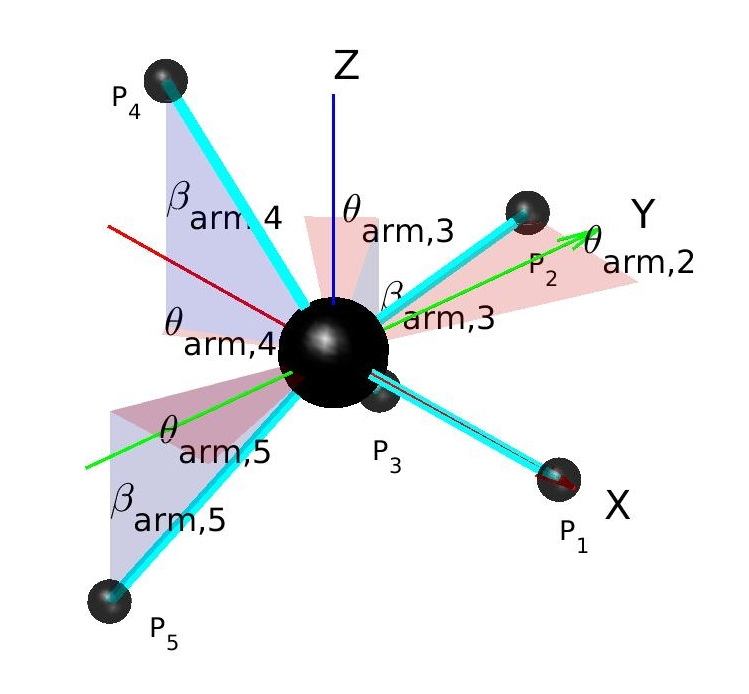
\includegraphics[width=\linewidth]{images/Pentacopter_odd.jpg}
    \caption{Optimal penta-copter.} \label{fig:Pentacopter_odd}
  \end{subfigure}
  \hspace*{\fill} % separation between the subfigures
  \begin{subfigure}[b]{0.55\textwidth}
    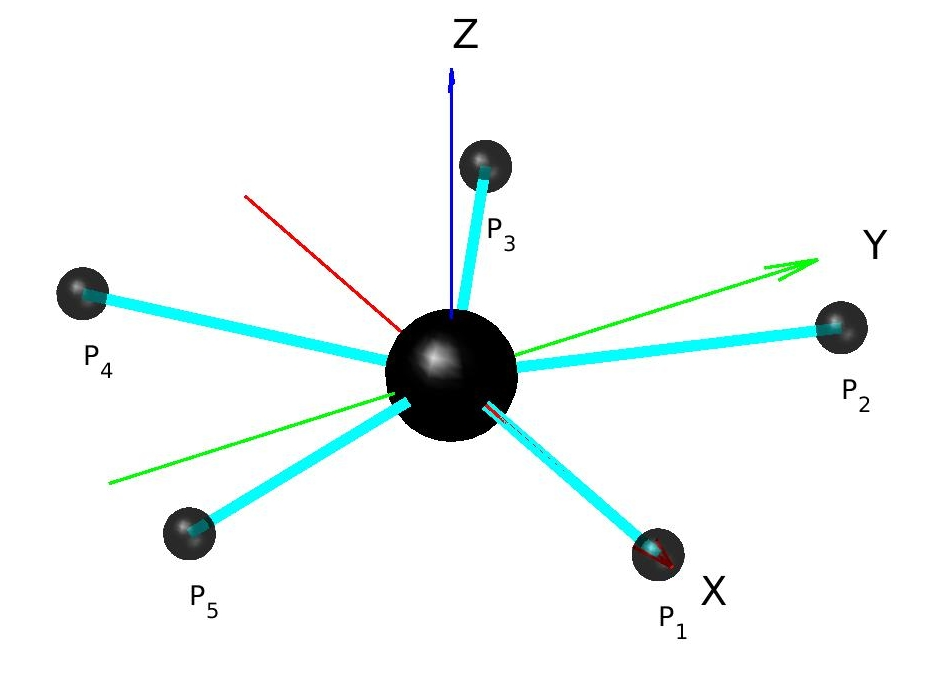
\includegraphics[width=\linewidth]{images/Pentacopter_standard.jpg}
    \caption{Penta-copter standard.} \label{fig:Pentacopter_standard}
  \end{subfigure}
  \caption{Schematic of different possible designs for a Penta-copter.}
  \label{fig:Pentacopter_result}
\end{figure}

Even though in this optimal penta-copter the arm angles seems very
peculiar, the propeller appear to be quite evenly disposed around the
MAV. Hence, when looking at  \Cref{fig:penta_fspace} and
\Cref{fig:penta_tspace} the force and torque spaces of the
optimal penta-copter are close to a sphere’s shape, and when
looking at \Cref{fig:penta_hspace} the hover efficiency
displayed by this design seems outstanding. And when
examining the values showed in \Cref{tab:tab_Penta_compare_force},
\Cref{tab:tab_Penta_compare_torque} and \Cref{tab:tab_Penta_compare_hover}
the first impression are confirmed, despite rather low minimal attainable
force and torque, this optimal design shows a very good average hover
efficiency.

\begin{table}[!ht]
\begin{center}
 \caption{Information on the designs’ force space properties.}\vspace{1ex}
 \label{tab:tab_Penta_compare_force}
 \resizebox{\textwidth}{!}{\begin{tabular}{|c|cccccc|}
 \hline
 Design & $F_{min}\ [N]$ & $F_{max}\ [N]$ & $F_{mean}\ [N]$ & $MAD(F)\ [N]$
 & Force space volume $[N^3]$& Force space surface $[N^2]$\\ \hline
 Optimal & 26.03 & 36.22 & 33.69 & 1.39 & 160'333 & 14'626\\
 Standard & 26.24 & 43.42 & 31.93 & 3.25 & 146'006 & 14'137\\
 \hline
 \end{tabular}}
\end{center}
\end{table}

\begin{table}[!ht]
\begin{center}
 \caption{Information on the designs’ torque space properties.}\vspace{1ex}
 \label{tab:tab_Penta_compare_torque}
 \resizebox{\textwidth}{!}{\begin{tabular}{|c|cccccc|}
 \hline
 Design & $M_{min}\ [Nm]$ & $M_{max}\ [Nm]$ & $M_{mean}\ [Nm]$ & $MAD(M)\ [Nm]$
 & Torque space volume $[N^3m^3]$ & Torque space surface $[N^2m^2]$\\ \hline
 Optimal & 12.85 & 18.2 & 16.93 & 0.7 & 20'358 & 3'741\\
 Standard & 10.9 & 21.8 & 16 & 1.63 & 18'409 & 3'580\\
 \hline
 \end{tabular}}
\end{center}
\end{table}

\begin{table}[!ht]
\begin{center}
 \caption{Information on the designs’ hover efficiency space properties.}\vspace{1ex}
 \label{tab:tab_Penta_compare_hover}
  {\scriptsize\begin{tabular}{|c|cccc|}
 \hline
  Design & $H_{eff,min}\ [\%]$ & $H_{eff,max}\ [\%]$ & $H_{eff,mean}\ [\%]$
  & $MAD(H_{eff})\ [\%]$\\ \hline
  Optimal & 80.33 & 99.4 & 90.96 & 3\\
  Standard & 77.25 & 100 & 84.38 & 5.2\\
 \hline
\end{tabular}}
\end{center}
\end{table}

\begin{figure}[!ht]
  \resizebox{\textwidth}{!}{\begin{subfigure}[b]{0.5\textwidth}
    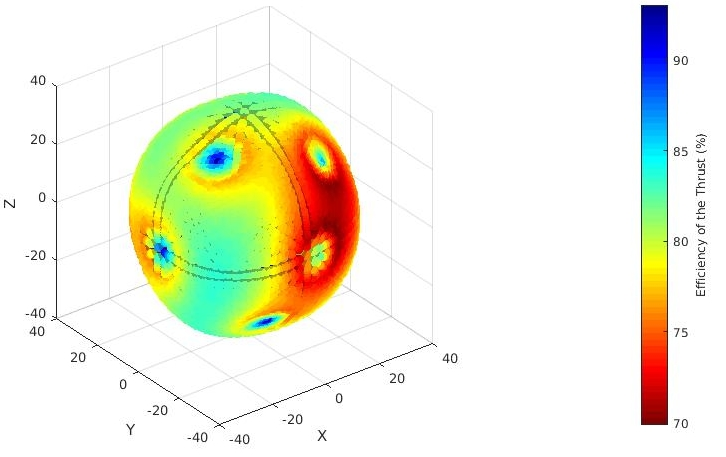
\includegraphics[width=\linewidth]{images/Penta_fspace.jpg}
    \caption{Attainable force space.} \label{fig:penta_fspace}
  \end{subfigure}
  \hspace*{\fill} % separation between the subfigures
  \begin{subfigure}[b]{0.45\textwidth}
    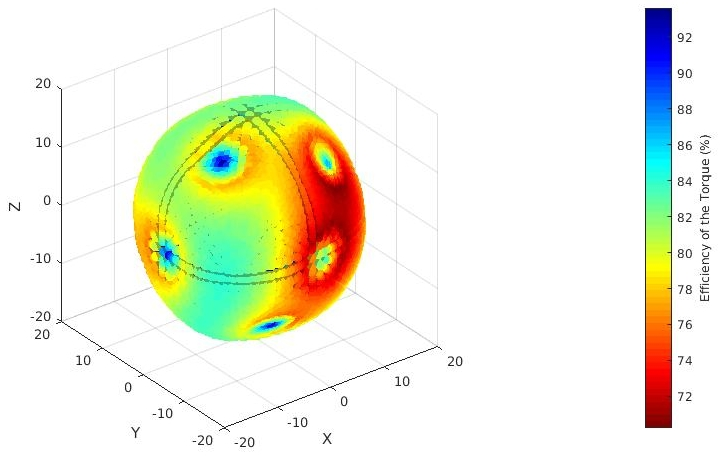
\includegraphics[width=\linewidth]{images/Penta_tspace.jpg}
    \caption{Attainable torque space.} \label{fig:penta_tspace}
  \end{subfigure}
  \begin{subfigure}[b]{0.5\textwidth}
    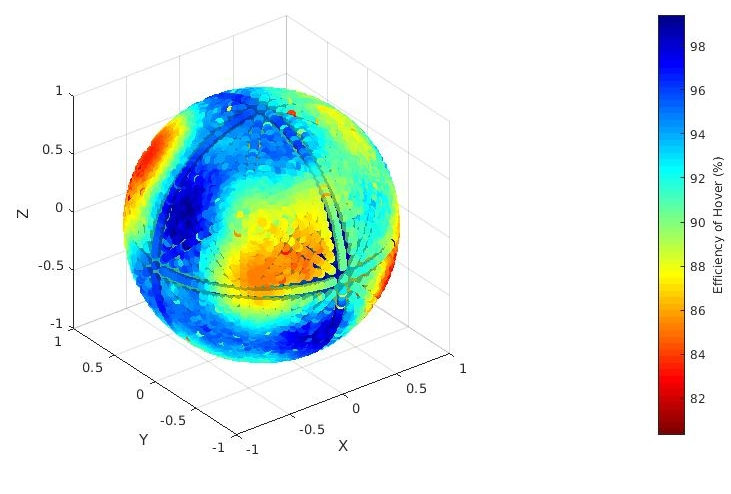
\includegraphics[width=\linewidth]{images/Penta_hspace.jpg}
    \caption{Hover efficiency in every orientation.} \label{fig:penta_hspace}
  \end{subfigure}}
  \caption{Visual representation of the abilities of the optimal penta-copter.}
  \label{fig:Pentacopter_spaces}
\end{figure}

\begin{figure}[!ht]
  \resizebox{\textwidth}{!}{\begin{subfigure}[b]{0.55\textwidth}
    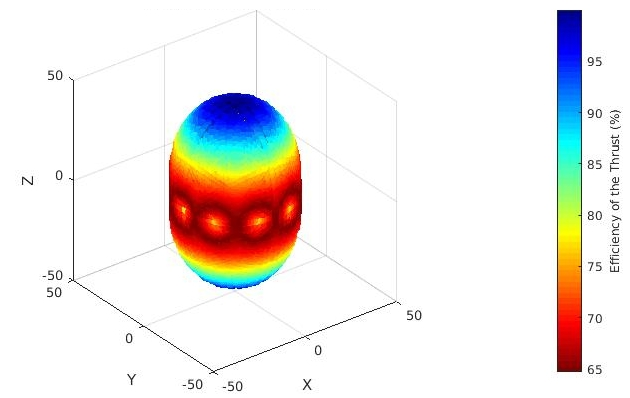
\includegraphics[width=\linewidth]{images/Penta_standard_fspace.jpg}
    \caption{Attainable force space.} \label{fig:penta_standard_fspace}
  \end{subfigure}
  \hspace*{\fill} % separation between the subfigures
  \begin{subfigure}[b]{0.5\textwidth}
    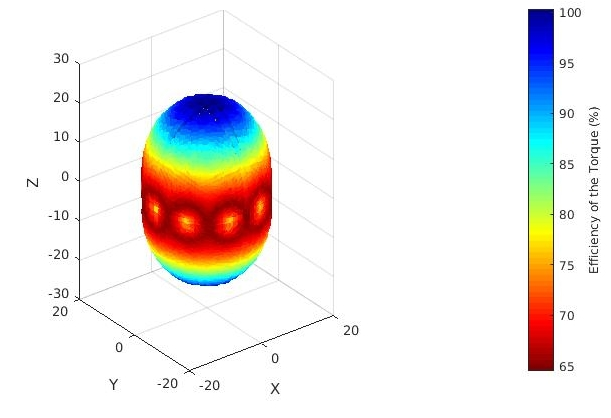
\includegraphics[width=\linewidth]{images/Penta_standard_tspace.jpg}
    \caption{Attainable torque space.} \label{fig:penta_standard_tspace}
  \end{subfigure}
  \begin{subfigure}[b]{0.45\textwidth}
    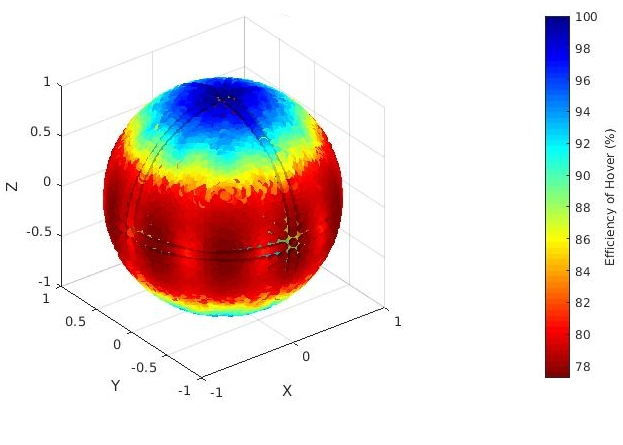
\includegraphics[width=\linewidth]{images/Penta_standard_hspace.jpg}
    \caption{Hover efficiency in every orientation.} \label{fig:penta_standard_hspace}
  \end{subfigure}}
  \caption{Visual representation of the abilities of the standard penta-copter.}
  \label{fig:penta_standard_spaces}
\end{figure}

\subsection{Hepta-copter}
\label{sec:hepta_copter}

The last design of this section is a very interesting design. Once more optimizing
the arm angles in order to obtain the maximal minimum attainable force and torque,
this result was obtained from the tool. The design is represented in
\Cref{fig:Heptacopter}and is defined by:

{\scriptsize\begin{itemize}
  \item $n\ =\ 7$
  \item $\beta_{arm}\ =\ [35.26^{\circ},\  35.26^{\circ},\  35.26^{\circ},\  35.26^{\circ},\
                          35.26^{\circ},\  35.26^{\circ},\  35.26^{\circ}]$
  \item $\theta_{arm}\ =\ [0^{\circ},\  0^{\circ},\  0^{\circ},\  0^{\circ},\  0^{\circ},\
                            0^{\circ},\  0^{\circ}]$
  \item $L\ =\ 0.5\ [m]$
\end{itemize}}

The $\beta_{arm}$ fully converged to the $\beta_{PS}$ angle, but in contrast with the
optimal designs with an even number of propeller, this optimal design have all its arms
oriented downwards. As explained in \Cref{sec:quad_copter}, the designs with the arms
oriented of $\beta_{PS}$ downwards and the design with the arms alternatively oriented
of $\beta_{PS}$ upwards and downwards are equivalent (for an even number of propeller).
The only difference is a change in the CoM position. However, for the designs with an odd
number of propellers, the arms can not be alternatively oriented of $\beta_{PS}$ upwards
and downwards. This would lead to two consecutive arms tilted downwards or upwards
and thus an unbalanced design. However, despite the control inconvenience due to the
CoM offset, this hepta-copter optimal design is very interesting, because the arms
oriented downwards would leave place on the top of the MAV for a manipulator with
a descent task space. Furthermore, when analyzing this design’s hover efficiency space
in \Cref{fig:Hepta_hspace} one can notice that except when the drone is in its initial
position as in \Cref{fig:Heptacopter}), the drone displays a very good hover efficiency.
It would thus be a perfect design for aerial manipulation.

\begin{figure}[!ht]
  \begin{center}
    \resizebox{\textwidth}{!}{\begin{subfigure}[b]{0.4\textwidth}
      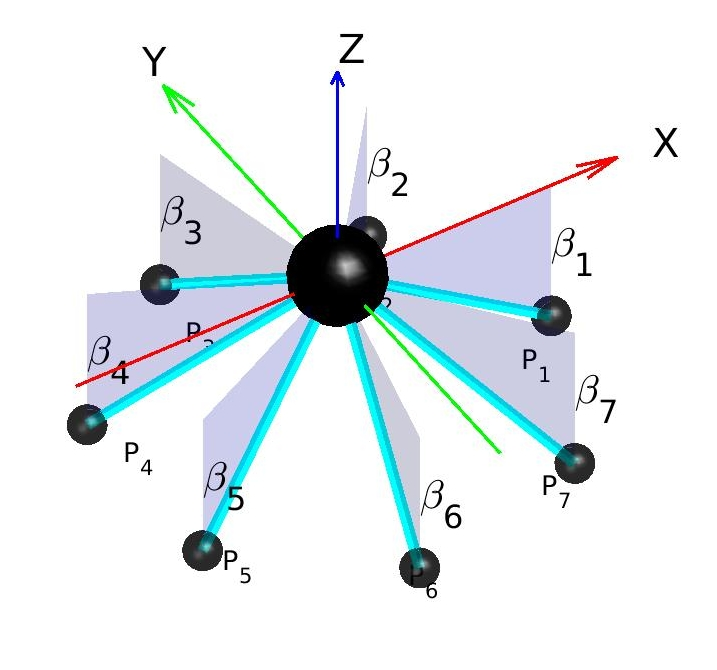
\includegraphics[width=\linewidth]{images/Heptacopter.jpg}
      \caption{Hover efficiency space.} \label{fig:Heptacopter}
    \end{subfigure}
    \hspace*{\fill} % separation between the subfigures
    \begin{subfigure}[b]{0.45\textwidth}
      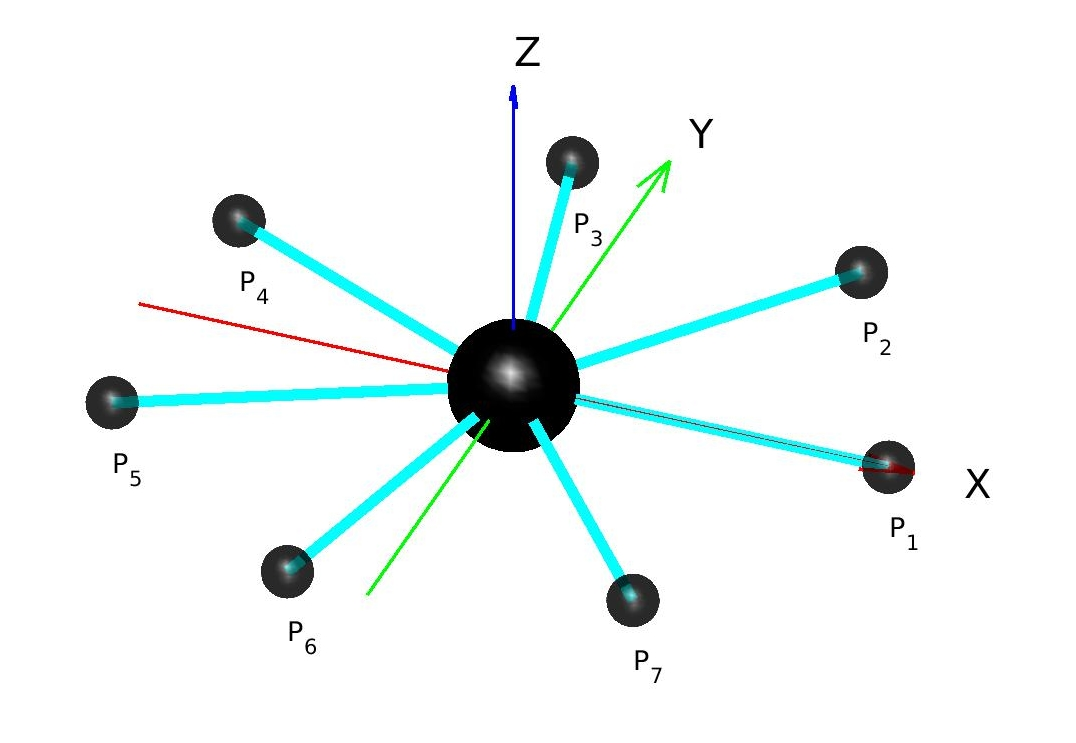
\includegraphics[width=\linewidth]{images/Heptacopter_standard.jpg}
      \caption{Hover efficiency space.} \label{fig:Heptacopter_standars}
    \end{subfigure}}
    \resizebox{\textwidth}{!}{\begin{subfigure}[b]{0.5\textwidth}
      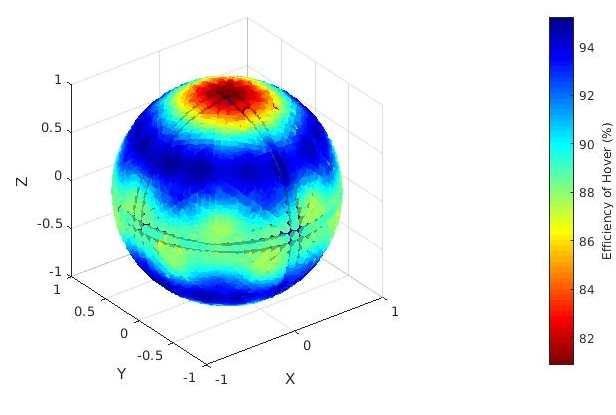
\includegraphics[width=\linewidth]{images/Hepta_opt_hspace.jpg}
      \caption{Optimal design hover efficiency space.} \label{fig:Hepta_opt_hspace}
    \end{subfigure}
    \hspace*{\fill} % separation between the subfigures
    \begin{subfigure}[b]{0.5\textwidth}
      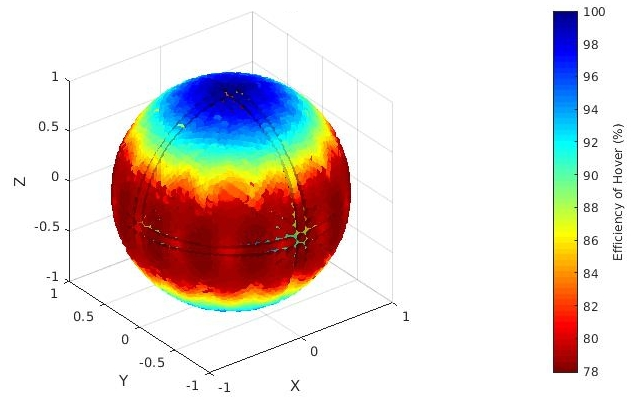
\includegraphics[width=\linewidth]{images/Hepta_hspace.jpg}
      \caption{Standard design hover efficiency space.} \label{fig:Hepta_hspace}
    \end{subfigure}}
    \caption{Visual representation of the optimal Hepta-copter capabilities.}
    \label{fig:Heptacopter_result}
  \end{center}
\end{figure}

\section{Comparison of Different Designs}
\label{sec:comparison}

From the results discussed above, it is possible to draw a general law on the
 omni-directional MAVs with tilting rotors. Indeed, the design of a n-rotors
MAV is optimally omni-drectional when the arms of the drone are evenly
distributed on the horizontal plane, and when they all form an angle of
$|\beta|\ =\ 35.26^{\circ}$ with the same horizontal plane. Furthermore, the
$\beta$ angles have to be alternatively oriented upwards and downwards if n
is even, or all oriented downwards if n is odd. The designs arising from this
law for $n\ = \ 3$ to $n\ = \ 8$ are represented in \Cref{fig:Compare_all_regular_designs}
And the information on their abilities are shown in \Cref{tab:tab_all_compare_force},
\Cref{tab:tab_all_compare_torque} and \Cref{tab:tab_all_compare_hover}.
From there, depending on their needs, one can choose one of those designs.
For instance, if the aim is to do aerial manipulation with descent payloads the
hepta-copter seems to be ideal. In contrast with the hexa-copter, which would not
be the ideal design to mount a manipulator, but would perform well when filming or taking
picture in any position at any orientation for as an example bridge inspection or film
making.

\begin{figure}[!ht]
  \resizebox{\textwidth}{!}{\begin{subfigure}[b]{0.5\textwidth}
    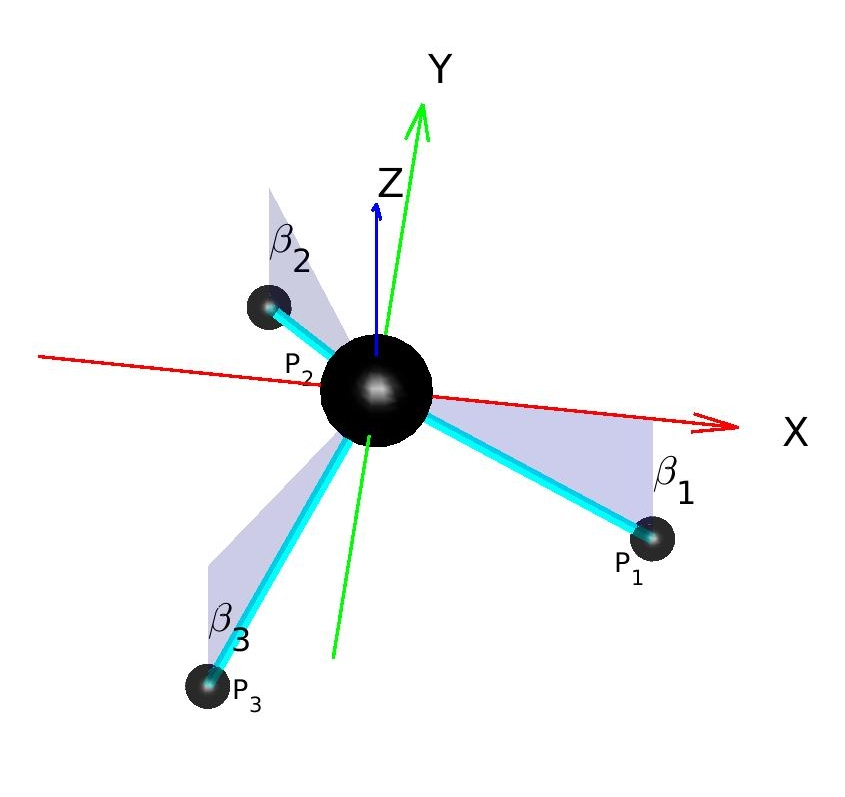
\includegraphics[width=\linewidth]{images/Tricopter.jpg}
    \caption{Tri-copter.} \label{fig:comp_tri}
  \end{subfigure}
  \hspace*{\fill} % separation between the subfigures
  \begin{subfigure}[b]{0.5\textwidth}
    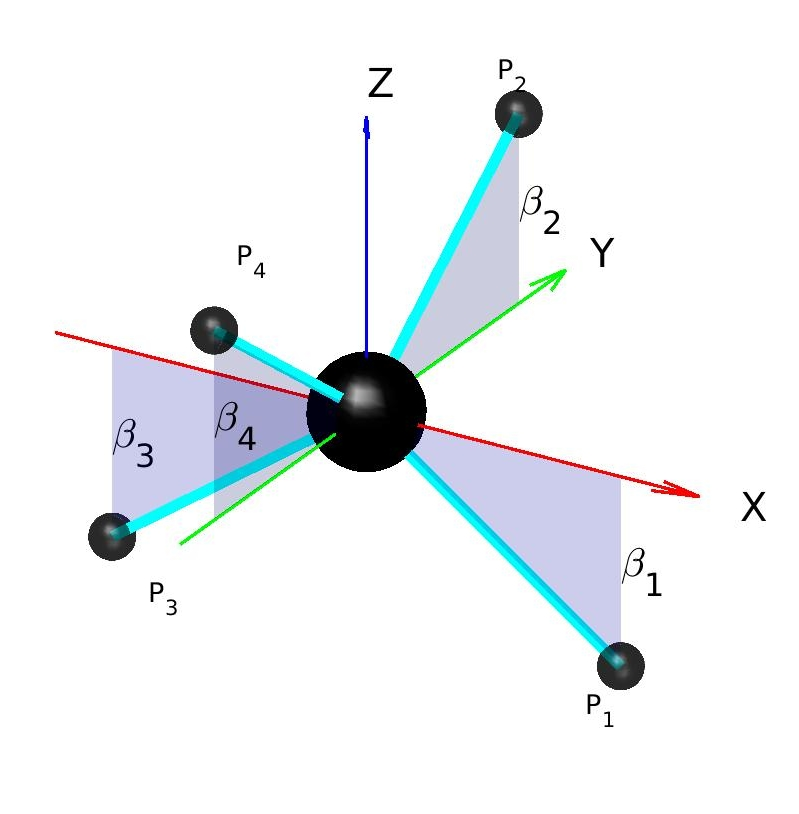
\includegraphics[width=\linewidth]{images/Quadcopter.jpg}
    \caption{Quad-copter.} \label{fig:comp_quad}
  \end{subfigure}
  \begin{subfigure}[b]{0.5\textwidth}
    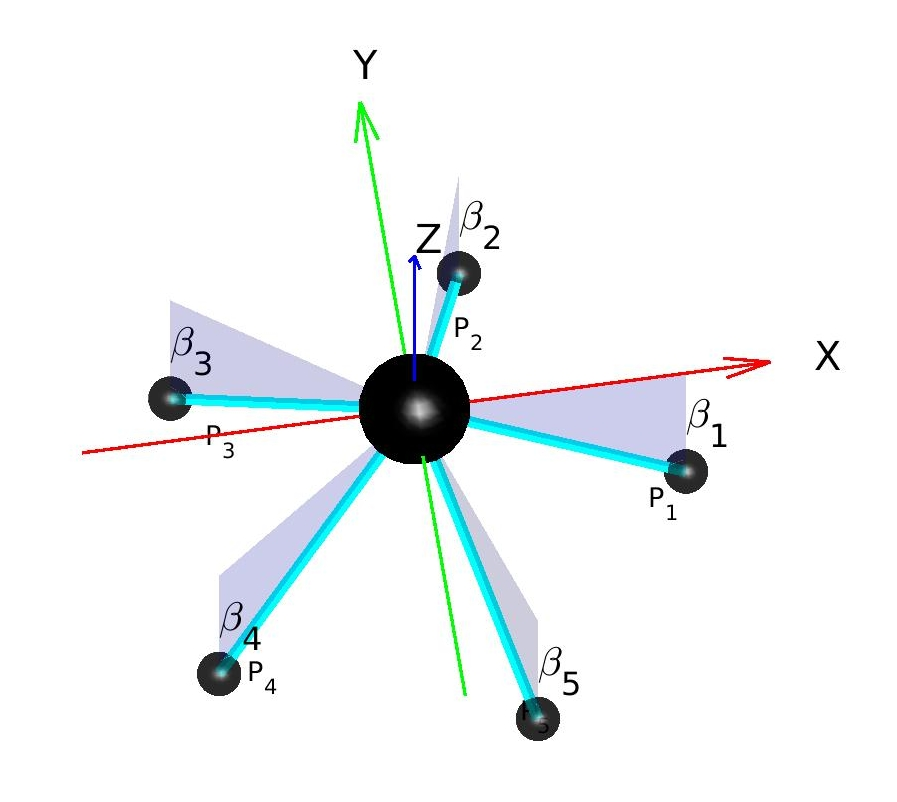
\includegraphics[width=\linewidth]{images/Pentacopter.jpg}
    \caption{Penta-copter.} \label{fig:comp_penta}
  \end{subfigure}}
  \resizebox{\textwidth}{!}{\begin{subfigure}[b]{0.5\textwidth}
    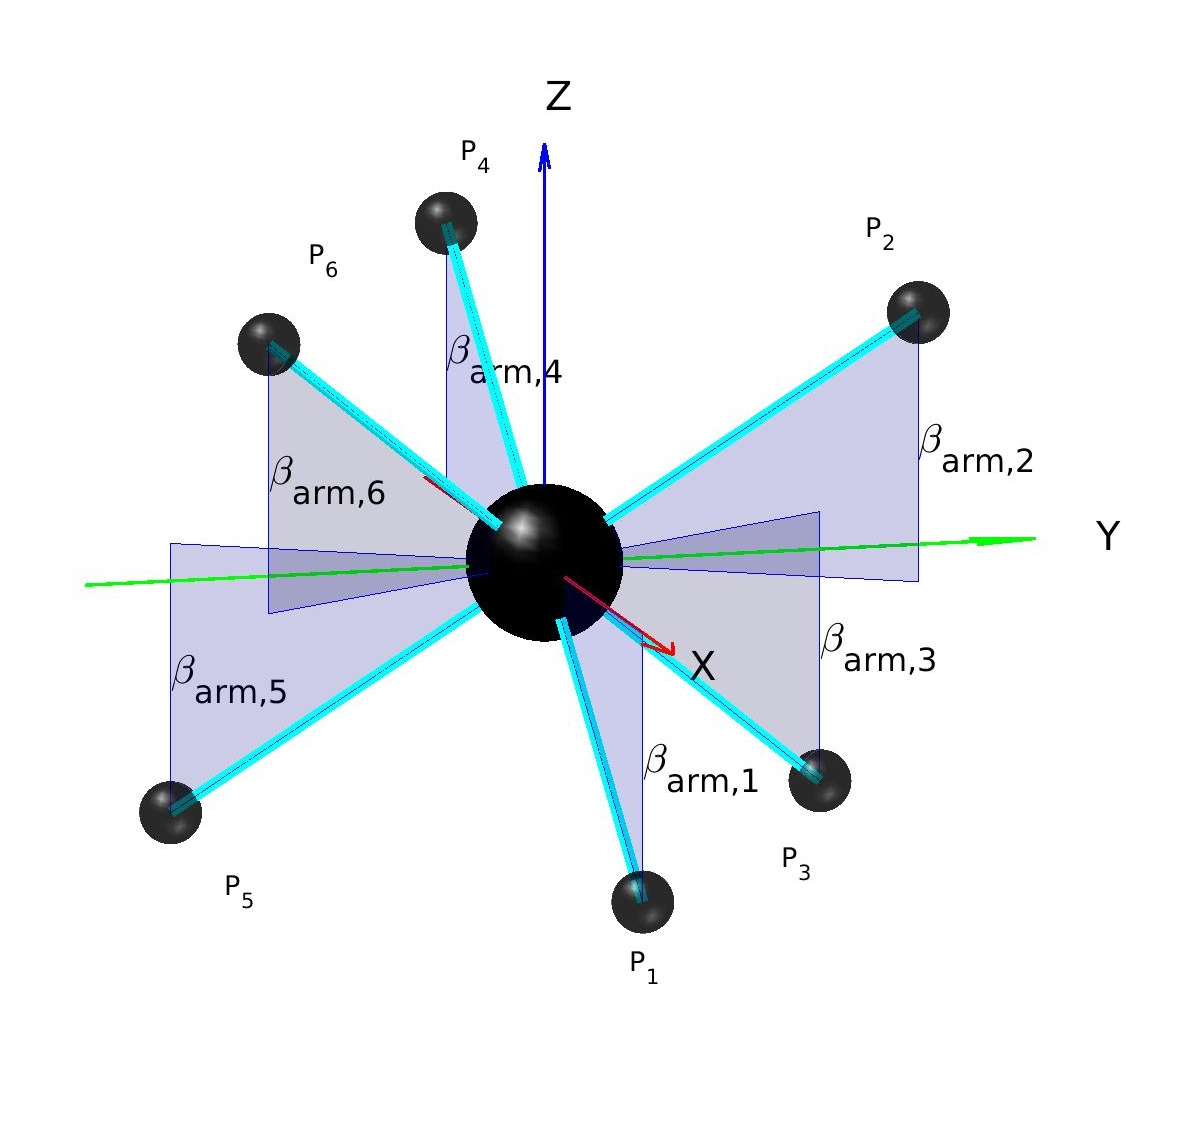
\includegraphics[width=\linewidth]{images/Hexacopter.jpg}
    \caption{Hexa-copter.} \label{fig:comp_hexa}
  \end{subfigure}
  \hspace*{\fill} % separation between the subfigures
  \begin{subfigure}[b]{0.5\textwidth}
    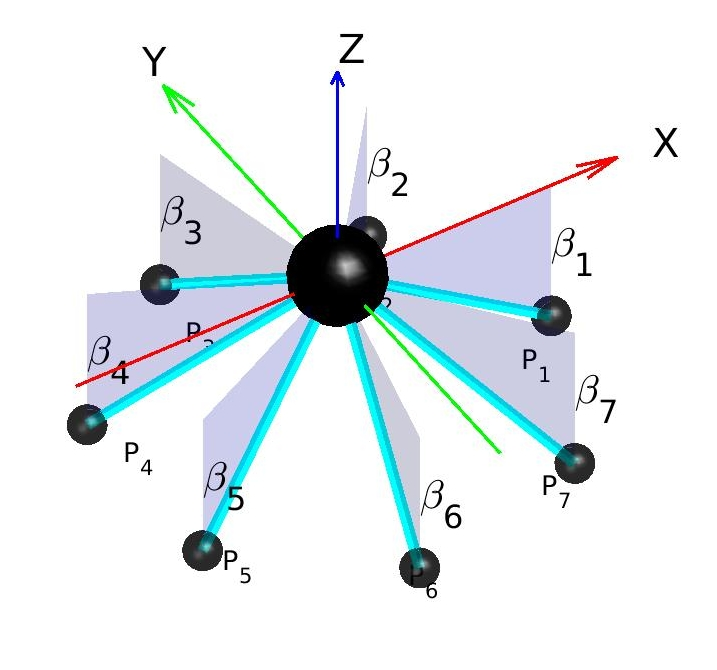
\includegraphics[width=\linewidth]{images/Heptacopter.jpg}
    \caption{Hepta-copter.} \label{fig:comp_hepta}
  \end{subfigure}
  \begin{subfigure}[b]{0.5\textwidth}
    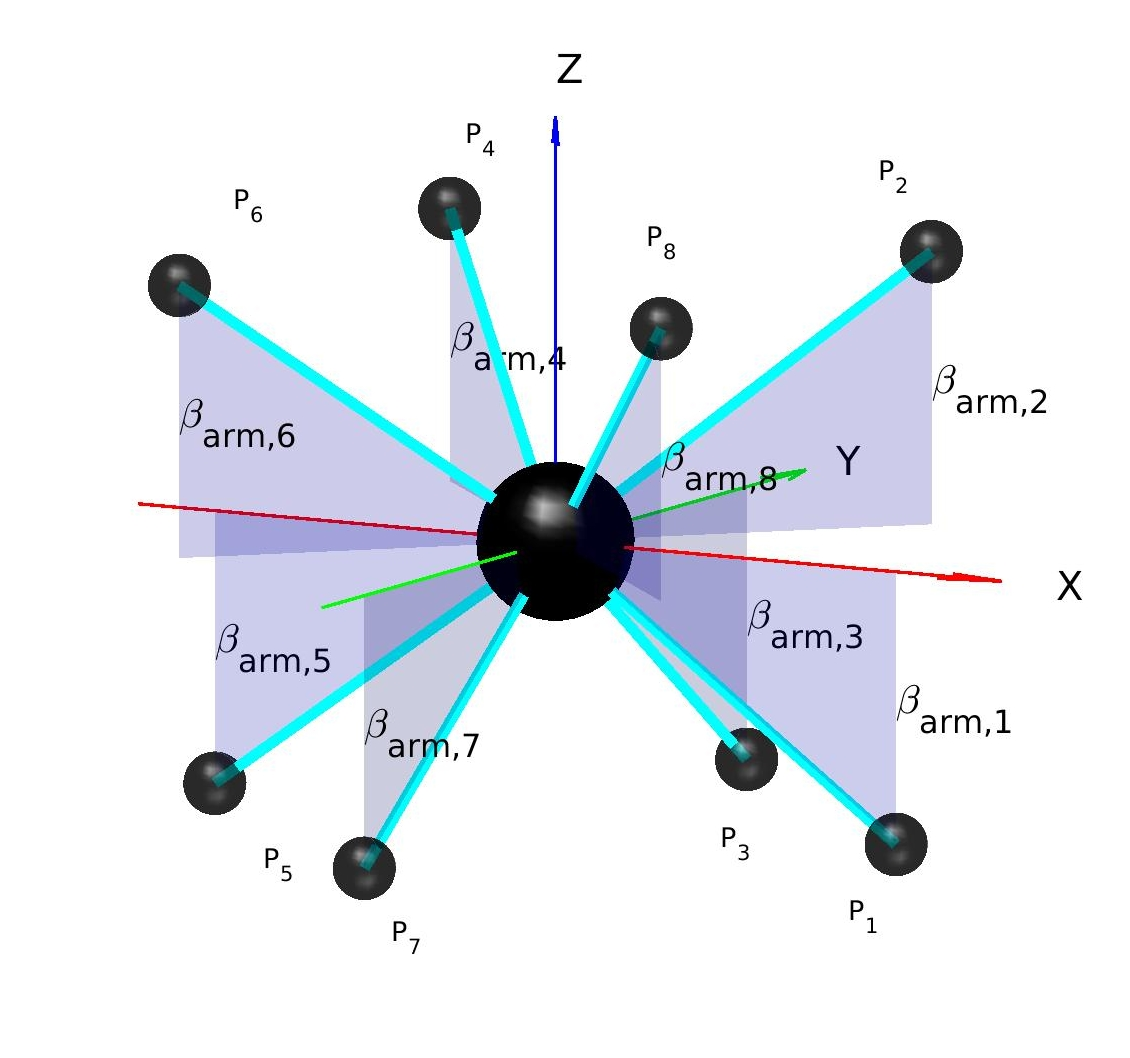
\includegraphics[width=\linewidth]{images/Octacopter.jpg}
    \caption{Octa-copter.} \label{fig:comp_octo}
  \end{subfigure}}
  \caption{Representation of all the optimal designs.}
  \label{fig:Compare_all_regular_designs}
\end{figure}

\begin{table}[!ht]
  \begin{center}
   \caption{Comparison between all the different optimal designs' force space properties.}\vspace{1ex}
   \label{tab:tab_all_compare_force}
   \resizebox{\textwidth}{!}{\begin{tabular}{|l|cccccc|}
     \hline
     Design & $F_{min}\ [N]$ & $F_{max}\ [N]$ & $F_{mean}\ [N]$ & $MAD(F)\ [N]$
     & Force space volume $[N^3]$& Force space surface $[N^2]$\\ \hline
     Tri-copter &  17.37 & 21.27 & 19.73 & 1.1 & 33'217 & 5'313\\
     Quad-copter & 23.23 & 28.37 & 26.87 & 0.86 & 81'710 & 9'326\\
     Penta-copter & 28.95 & 35.46 & 29.39 & 0.46 & 107'463 & 11'130\\
     Hexa-copter & 34.74 & 42.55 & 39.52 & 2.21 & 267'010 & 20'922\\
     Hepta-copter & 39.96 & 49.44 & 47.18 & 0.96 & 447'344 & 28'929\\
     Octa-copter & 44.7 & 58.78 & 53.95 & 0.94 & 669'339 & 37'625\\
     \hline
   \end{tabular}}
  \end{center}
\end{table}

\begin{table}[!ht]
  \begin{center}
   \caption{Comparison between all the different optimal designs' torque space properties.}\vspace{1ex}
   \label{tab:tab_all_compare_torque}
   \resizebox{\textwidth}{!}{\begin{tabular}{|l|cccccc|}
     \hline
     Design & $M_{min}\ [Nm]$ & $M_{max}\ [Nm]$ & $M_{mean}\ [Nm]$ & $MAD(M)\ [Nm]$
     & Torque space volume $[N^3m^3]$ & Torque space surface $[N^2m^2]$\\ \hline
     Tri-copter & 8.7 & 10.67 & 9.87 & 0.56 & 4'158 & 1'379\\
     Quad-copter & 11.65 & 14.23 & 13.47 & 0.43 & 10'300 & 2'348\\
     Penta-copter & 14.52 & 17.78 & 14.74 & 0.23 & 13'555 & 2'800\\
     Hexa-copter & 17.42 & 21.34 & 19.82 & 1.1 & 33'687 & 5'230\\
     Hepta-copter & 20.04 & 24.8 & 23.66 & 0.48 & 56'403 & 7'304\\
     Octa-copter & 22.4 & 29.48 & 27 & 0.47 & 84'417 & 9'463\\
     \hline
   \end{tabular}}
  \end{center}
\end{table}

\begin{table}[!ht]
  \begin{center}
   \caption{Comparison between all the different optimal designs' hover efficiency space properties.}\vspace{1ex}
   \label{tab:tab_all_compare_hover}
     {\scriptsize\begin{tabular}{|l|cccc|}
       \hline
        Design & $H_{eff,min}\ [\%]$ & $H_{eff,max}\ [\%]$ & $H_{eff,mean}\ [\%]$
        & $MAD(H_{eff})\ [\%]$\\ \hline
        Tri-copter & 81.65 & 99 & 87.22 & 4.42\\
        Quads-copter & 81.65 & 94.73 & 87.1 & 2.6\\
        Penta-copter & 81.65 & 91.43 & 85.35 & 1.49\\
        Hexa-copter & 81.65 & 100 & 88.92 & 4.43\\
        Hepta-copter & 80.88 & 95.23 & 91.1 & 2.4 \\
        Octa-copter & 81.78 & 96.65 & 91.42 & 2.7\\
       \hline
    \end{tabular}}
  \end{center}
\end{table}
